%\pdfminorversion=5  %por la version de los pdf que incluyo
\documentclass[spanish,a4paper,12pt]{article}

\usepackage[utf8]{inputenc}
\usepackage[T1]{fontenc}
\usepackage[spanish]{babel}

\usepackage{graphicx}
%\usepackage{eurosym}
\usepackage{epstopdf}
\usepackage{anysize}
\usepackage[indent,bf]{caption}
\usepackage{fancyhdr}
\setlength{\headheight}{27.2pt}
\addtolength{\topmargin}{-11.7pt}
\pagestyle{fancy}
\usepackage{amsmath,amssymb}
\usepackage{tikz,pgfplots}
\usetikzlibrary{arrows,shapes}
\usepackage[matrix,arrow]{xy}
\usepackage{array}
\usepackage{subcaption}
\usepackage{float}
\usepackage{pdfpages}

\usepackage[toc,acronym,nonumberlist]{glossaries}
\makeglossaries

\newacronym{5g}{5G}{Fifth Generation Mobile Network}
\newacronym{5ga}{5GA}{5G-Advanced}
\newacronym{nsa}{NSA}{Non-Standalone}
\newacronym{sa}{SA}{Standalone}
\newacronym{5gnsa}{5G NSA}{5G Non-Standalone}
\newacronym{5gsa}{5G SA}{5G Standalone}
\newacronym{can}{CAN}{Controller Area Network}
\newacronym{dds}{DDS}{Data Distribution Service}
\newacronym{iot}{IoT}{Internet of Things}
\newacronym{iteamupv}{iTEAM-UPV}{Instituto de Telecomunicaciones y Aplicaciones Multimedia}
\newacronym{lidar}{LiDAR}{Light Detection and Ranging}
\newacronym{omg}{OMG}{Object Management Group}
\newacronym{ptz}{PTZ}{Pan-Tilt-Zoom}
\newacronym{qos}{QoS}{Quality of Service}
\newacronym{ran}{RAN}{Radio Access Network}
\newacronym{ros}{ROS}{Robot Operating System}
\newacronym{ros1}{ROS 1}{Robot Operating System 1}
\newacronym{ros2}{ROS 2}{Robot Operating System 2}
\newacronym{ues}{UEs}{User Equipments}
\newacronym{upv}{UPV}{Universidad Politécnica de Valencia}
\newacronym{mimo}{MIMO}{Massive Input Massive Output}
\newacronym{cu}{CU}{Centralized Unit}
\newacronym{du}{DU}{Descentralized Unit}
\newacronym{ru}{RU}{Remote Unit}
\newacronym{tdd}{TDD}{Time Division Duplex}
\newacronym{upf}{UPF}{User Platform Function}
\newacronym{e2e}{E2E}{End to End}
\newacronym{slam}{SLAM}{Simultaneous Localization and Mapping}
\newacronym{sba}{SBA}{Service--Base Architecture}
\newacronym{nfv}{NFV}{Network Function Virtualization}
\newacronym{cu_du_ru}{CU--DU--RU}{Centralized Unit -- Distributed Unit -- Remote Unit}
\newacronym{tcp}{TCP}{Transmission Control Protocol}
\newacronym{udp}{UDP}{User Datagram Protocol}
\newacronym{raplet}{RAPLET}{ROS-Aware Publish/Subscribe Latency Evaluation Tool}
\newacronym{ia}{IA}{inteligencia artificial}
\newacronym{5qi}{5QI}{5G QoS Identifier}
\newacronym{3gpp}{3GPP}{3rd Generation Partnership Project}




\usepackage[colorlinks,bookmarks=true,bookmarksnumbered=false,
linkcolor=black,citecolor=black]{hyperref}

\pgfplotscreateplotcyclelist{mylist2}{%
{blue!60!black,mark=*,mark repeat=5,mark size=1,7,line width=1},
{red!60!black,mark=square*,mark repeat=5,mark size=0.6,line width=1}}

\pgfplotscreateplotcyclelist{mylist3}{%
{blue!60!black,mark=*,mark repeat=5,mark size=0.7,line width=1},
{red!60!black,mark=square*,mark repeat=5,mark size=0.6,line width=1},
{green!50!black,mark=diamond*,mark repeat=5,mark size=0.9,line width=1}}


\pgfplotscreateplotcyclelist{mylist6}{%
{blue!60!black,mark=*,mark repeat=5,mark size=0.7,line width=1},
{red!60!black,mark=*,mark repeat=5,mark size=0.7,line width=1},
{green!50!black,mark=*,mark repeat=5,mark size=0.7,line width=1},
{blue!40!black!40!white,mark=square*,mark repeat=5,mark size=0.8,line width=1},
{red!40!black!40!white,mark=square*,mark repeat=5,mark size=0.8,line width=1},
{green!40!black!40!white,mark=square*,mark repeat=5,mark size=0.8,line width=1}}

\marginsize{2.5cm}{2.5cm}{2cm}{3cm} % Controla los márgenes {izquierda}{derecha}{arriba}{abajo}. 
 
\setlength{\headheight}{15.5pt}

 \pagestyle{fancyplain}
 \lhead[\fancyplain{}{\bf \thepage}]{\fancyplain{}{\bf \rightmark}}
 \rhead[\fancyplain{}{\bf \leftmark}]{\fancyplain{}{\bf \thepage}}
 \chead{} \lfoot{} \cfoot{\fancyplain{}{}} \rfoot{}

\renewcommand{\sectionmark}[1]{\markboth{#1}{#1}}
 
\newcommand{\estilouno}{\bf \em \color{blue!70!black}}

\newcommand{\estilodos}{\bf \color{blue!70!black}}

\begin{document}

\renewcommand{\tablename}{Tabla}

% Escribir aquí el título del trabajo fin de máster
\newcommand{\titul}{Análisis experimental de aplicaciones robóticas basadas en ROS sobre una infraestructura 5G}
% ------------------
\sectionmark{\titul}

%\input{titul} NO INCLUYO LA PORTADA
\cleardoublepage
\thispagestyle{fancyplain}
\setcounter{page}{1}



\newpage

\vspace{1cm}

\noindent {\estilouno Objetivos -- }

De forma más concreta:
\begin{enumerate}

\item \textbf{Caracterización del modelo \gls{ros1} integrado por Summit XL}

Analizar la arquitectura de comunicación de \gls{ros1} integrada por la plataforma Summit XL, con el fin de identificar los procesos mas demansantes.

\item \textbf{Selección e integración de herramientas de medición}

Investigar herramientas existentes para la medición de latencias y otros parámetros de rendimiento en \gls{ros1}, seleccionar una herramienta adecuada e integrarla en el entorno experimental para la obtención de métricas cuantitativas.

\item \textbf{Diseño de arquitectura distribuida Robot--Edge}

Diseñar una arquitectura distribuida mínima que represente un escenario Robot--Edge, constituida por nodos locales y nodos remotos desplegados en diferentes máquinas, permitiendo evaluar comunicaciones extremo a extremo en un entorno distribuido real.

\item \textbf{Evaluación bajo infraestructura \gls{5g}}

Configurar y utilizar una infraestructura de red \gls{5g} representativa de un entorno real, considerando parámetros como latencia, variabilidad temporal y pérdida de paquetes, con el fin de generar escenarios experimentales reproducibles.

\item \textbf{Análisis cuantitativo de las comunicaciones}

Medir y analizar cuantitativamente el comportamiento del sistema bajo distintas condiciones de red, evaluando parámetros como latencia end--to--end, tasa de transferencia, estabilidad de comunicación y diferencias entre ejecución local y distribuida.

\end{enumerate}


\vspace{3.5cm}

\noindent {\estilouno Metodología -- }  ...

\vspace{3.5cm}

\noindent {\estilouno Desarrollos teóricos realizados -- }  ...

\vspace{3.5cm}

\noindent {\estilouno Desarrollo de prototipos y trabajo de laboratorio -- }  ...

\vspace{3.5cm}

\noindent {\estilouno Resultados -- }  ...

\vspace{3.5cm}

\noindent {\estilouno Líneas futuras -- }  ...

\vspace{3.5cm}

\noindent {\estilouno Publicaciones -- } ...

\vspace{3.5cm}

\noindent {\estilouno Abstract -- }


\vspace{1em}

\noindent{\estilouno Resumen -- }




\vspace{3.5cm}

\vfill

\noindent Autor: Guillermo García Rodríguez, \href{mailto:guillegr1999@gmail.com}{email: guillegr1999@gmail.com} \\
Director: David Gomez-Barquero, \href{mailto:dagobar@iteam.upv.es}{email: dagobar@iteam.upv.es} \\
Tutor externo: Nuria Molner Siurana, \href{mailto:numolsiu@iteam.upv.es}{email: numolsiu@iteam.upv.es} \\
Tutor externo: Raúl Lozano Teruel, \href{mailto:raulote@iteam.upv.es}{email: raulote@iteam.upv.es} \\
Fecha de entrega: 31-05-26


\pagebreak 

\noindent {\estilodos LISTA DE ACRÓNIMOS -- }
\renewcommand{\glossarysection}[2][]{}
\printglossary[type=\acronymtype]

\vspace{3.5cm}

\noindent {\estilodos LISTA DE FIGURAS -- }
\renewcommand{\listfigurename}{}
\listoffigures

\pagebreak

\sectionmark{\titul}
\tableofcontents
\sectionmark{\titul}

\pagebreak

\sectionmark{\titul}

% ================================================================
% 01. INTRODUCCION
% ================================================================
\input{sections/01_introduccion/01_00_introduccion/01_00_00_introduccion}
\subsection{Contexto y motivación}
\label{sec:contexto_y_motivacion}

La robótica móvil está experimentando un crecimiento significativo en sectores como la industria o la logística. Los robots deben operar en entornos dinámicos y procesar grandes cantidades de información procedente de múltiples sensores. Tradicionalmente, los sistemas robóticos han sido diseñados para realizar las tareas computacionales de forma completamente local. Sin embargo, la creciente complejidad de las tareas ha puesto de manifiesto las limitaciones de esta estrategia, lo que ha impulsado el desarrollo de arquitecturas de computación distribuida que asisten con el procesamiento más allá de las limitaciones de los sistemas embarcados.

El paradigma de \textit{edge computing} ha emergido como una alternativa que permite trasladar parte del procesamiento a servidores cercanos, reduciendo la carga computacional del robot.

Paralelamente, las redes \gls{5g} ofrecen características especialmente adecuadas para sistemas robóticos distribuidos. Estas capacidades permiten establecer arquitecturas en las que los robots pueden intercambiar grandes volúmenes de datos con infraestructuras de computación externas en tiempo casi real, facilitando la distribución de tareas entre el robot y los servidores de \textit{edge computing}.

En este contexto, surge la necesidad de investigar metodologías que permitan distribuir de forma eficiente las funciones de un sistema robótico entre el robot y el \textit{edge}. Este tipo de arquitecturas híbridas plantea diversos desafíos, entre ellos la gestión de la latencia de comunicación, la selección de las tareas adecuadas para su ejecución remota y la integración de estas capacidades dentro de los middleware robóticos existentes.

El presente trabajo explora la integración de mecanismos de distribución de funciones entre el robot y el \textit{edge} en un sistema robótico basado en ROS desplegado sobre una red privada \gls{5g}.


% ================================================================
% 02. ESTADO DEL ARTE
% ================================================================
\section{Estado del arte}
\label{sec:estado_del_arte}

El desarrollo de sistemas robóticos conectados requiere la integración de infraestructuras de comunicaciones avanzadas, arquitecturas de computación distribuida y middleware robótico. En este capítulo se revisan los principales trabajos relacionados con redes \gls{5g} (Sección \ref{sec:arquitecturas_de_comunicacion_para_robotica_conectada}), \textit{edge computing} (Sección \ref{sec:edge_computing_para_sistemas_roboticos}), \textit{middleware} robótico (Sección \ref{sec:middleware_robotico_ros1_ros2}) y evaluación de latencia en sistemas robóticos distribuidos (Sección \ref{sec:evaluacion_de_latencia_en_sistemas_roboticos_distribuidos}).
\subsection{Arquitecturas de comunicación para robótica conectada}
\label{sec:arquitecturas_de_comunicacion_para_robotica_conectada}

El desarrollo del campo de la robótica móvil esta estrechamente vinculado al desarrollo de infraestructuras de comunicación capaces de soportar sistemas distribuidos y aplicaciones en tiempo real. Tradicionalmente, los robots móviles realizaban la mayor parte del procesamiento de forma local. Sin embargo, el creciente uso de sensórica, algoritmos de percepción basados en \gls{ia} y sistemas de control remoto ha incrementado significativamente las necesidades de computo.

En este contexto, las redes móviles \gls{5g} han emergido como una tecnología habilitadora de nuevas arquitecturas de robótica conectada. A diferencia de generaciones anteriores de redes móviles, el marco conceptual de \gls{5g} definido en IMT-2020 establece diferentes escenarios de servicio orientados a soportar aplicaciones con altos requisitos de capacidad, baja latencia y conectividad masiva de dispositivos \cite{3gppTS23501}. Estas capacidades permiten que robots móviles transmitan grandes volúmenes de datos procedentes de sensores y reciban comandos de control con tiempos de respuesta reducidos.

Desde el punto de vista arquitectónico, el sistema \gls{5g} se basa en un modelo denominado \gls{sba}, en el que las funciones de red se implementan como servicios modulares. Este enfoque facilita la virtualización de la red y la distribución flexible de funciones. Además, el sistema \gls{5g} introduce mecanismos como \textit{network slicing}, que permiten crear redes lógicas con características específicas para distintos servicios, y un modelo avanzado de \gls{qos} basado en identificadores \gls{5qi} para garantizar requisitos de latencia, fiabilidad y prioridad del tráfico. Asimismo, el estándar contempla el despliegue de \textit{Non-Public Networks} (NPN), que permiten operar infraestructuras \gls{5g} dedicadas para aplicaciones críticas \cite{3gppTS23501}.

Un ejemplo de red privadas \gls{5g} es la desplegada en el campus de la Universitat Politècnica de València, que proporciona cobertura interior y exterior mediante múltiples bandas de frecuencia y diferentes implementaciones del núcleo \gls{5g}, permitiendo la evaluación de diversos escenarios experimentales de conectividad \cite{ITEAM2025Private5G}. La red \gls{5gsa} del \gls{iteamupv} se describe con mayor detalle en la sección \ref{sec:capa_de_red_5g_privada}

El uso de redes \gls{5g} también facilita la transición hacia arquitecturas robóticas distribuidas, en las que determinadas funciones del sistema se ejecutan fuera de la plataforma robótica. Este enfoque permite reducir los requisitos de \textit{hardware} embarcado en el robot y mejorar la escalabilidad del sistema, aunque introduce nuevos retos relacionados con la latencia de comunicación, la estabilidad de los enlaces y la fiabilidad global de la red.

Diversos trabajos experimentales han explorado estas arquitecturas mediante plataformas de prueba que integran robots móviles con redes \gls{5g} privadas. En estos entornos, los robots transmiten flujos de datos sensoriales al \textit{edge} para su procesamiento y reciben información procesada para la toma de decisiones o la teleoperación. Los resultados muestran que el rendimiento del sistema depende de múltiples fuentes de latencia, incluyendo la transmisión de vídeo, el procesamiento de percepción asistido por \gls{ia} y el envío de comandos de control al robot \cite{Lozano2025DigitalTwin6G}.

En conjunto, estas investigaciones muestran que las redes \gls{5g} proporcionan la infraestructura necesaria para soportar arquitecturas robóticas distribuidas. No obstante, el comportamiento global del sistema depende de la interacción entre la red de comunicaciones, la arquitectura de procesamiento distribuido y el software robótico empleado. Por este motivo, el análisis del rendimiento de estos sistemas requiere considerar de forma conjunta las características de la red de comunicaciones y la distribución funcional de los componentes del sistema robótico.
\subsection{Edge computing para sistemas robóticos}
\label{sec:edge_computing_para_sistemas_roboticos}

El incremento en la cantidad de datos generados por sistemas robóticos modernos ha impulsado el desarrollo de arquitecturas de procesamiento distribuidas que permitan complementar las capacidades computacionales de los robots móviles. La ejecución local de estas tareas puede resultar limitada por las limitaciones de potencia de procesamiento y consumo energético de los sistemas embarcados.

En este contexto, el paradigma de \textit{edge computing} propone trasladar parte del procesamiento de datos desde los dispositivos finales hacia nodos de computación situados en el borde de la red. Estos nodos, denominados \textit{edge servers}, permiten ejecutar tareas computacionalmente más demandantes. Su proximidad a la fuente de datos reduce la latencia de comunicación respecto a los centros de datos (\textit{cloud}), lo que se traduce en menores tiempos de respuesta para aplicaciones sensibles al retardo.

Este tipo de configuraciones suele describirse como arquitecturas \textit{Robot--Edge--Cloud}, en las que las tareas de control y adquisición de datos se ejecutan en el robot, mientras que el procesamiento intensivo se desplaza hacia nodos de computación en el borde de la red o infraestructuras \textit{cloud}. Este enfoque permite reducir la carga computacional en la plataforma robótica, facilita el despliegue de aplicaciones más complejas y mejora la escalabilidad del sistema.

La integración de capacidades de computación en el borde de la red ha sido considerada en la evolución de las arquitecturas \gls{5g} . En particular, los trabajos de estandarización del \gls{3gpp} han analizado diferentes arquitecturas para habilitar aplicaciones desplegadas en el borde de la red y facilitar la interacción entre los dispositivos finales y los servidores de \textit{edge computing} \cite{3gppTR23758}. 

Plataformas experimentales basadas en redes privadas \gls{5g} han demostrado la viabilidad de integrar robots móviles con infraestructuras de computación distribuida en entornos industriales. Esto abre nuevas posibilidades para la optimización de procesos \cite{10885713}.

No obstante, la adopción de arquitecturas robóticas basadas en \textit{edge computing} plantea diversos retos técnicos, entre los que destacan la gestión de la latencia de comunicación, la asignación dinámica de recursos de computación y la coordinación entre los distintos componentes distribuidos del sistema. Por este motivo, el diseño de sistemas robóticos distribuidos requiere considerar conjuntamente las capacidades de la red de comunicaciones, la arquitectura de procesamiento y los requisitos temporales de las aplicaciones robóticas.
\subsection{Middleware robótico: ROS 1 y ROS 2}
\label{sec:middleware_robotico_ros1_ros2}

El desarrollo de sistemas robóticos modernos requiere de software capaz de gestionar la interoperabilidad entre componentes heterogéneos. En este contexto, los \textit{middleware} robóticos proporcionan una capa de abstracción que facilita la integración de elementos dentro de una arquitectura modular. Entre las distintas soluciones propuestas, \gls{ros} se ha consolidado como uno de los marcos de desarrollo más utilizados en investigación y aplicaciones robóticas.

\gls{ros} proporciona un conjunto de herramientas y bibliotecas para la construcción de aplicaciones robóticas mediante la orquestación de módulos independientes denominados \textit{nodes}. Estos nodos intercambian información a través de un modelo de comunicación basado en el paradigma \textit{publish–subscribe}, en el que los productores de datos publican información en canales denominados \textit{topics}, mientras que los consumidores se suscriben a dichos canales para recibir los mensajes correspondientes. Este modelo facilita el desacoplamiento entre los distintos componentes del sistema y permite desarrollar arquitecturas robóticas distribuidas \cite{ros_concepts}. La figura \ref{fig:ros_basic_concepts} muestra la relación  de estos elementos.

\begin{figure}[H]
    \centering
    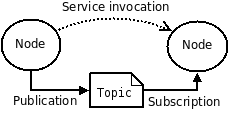
\includegraphics[width=0.35\linewidth]{figures/ROS_basic_concepts.png}
    \caption{Interacción entre elementos de ROS \cite{ros_concepts}}
    \label{fig:ros_basic_concepts}
\end{figure}

La primera generación del sistema, conocida como \gls{ros1}, la comunicación entre nodos se implementa mediante mecanismos de transporte basados en los protocolos de red \gls{tcp} y \gls{udp}, a través de las implementaciones TCPROS y UDPROS. Aunque esta arquitectura ha demostrado ser eficaz, presenta ciertas limitaciones en términos de escalabilidad y soporte para aplicaciones con requisitos estrictos de tiempo real. En particular, la latencia de comunicación entre nodos puede verse afectada por factores como el tamaño de los mensajes, la carga del sistema o las características de la red subyacente \cite{nishimura2021raplet}.

Con el objetivo de superar estas limitaciones, la segunda generación del \textit{framework}, \gls{ros2}, introduce una arquitectura de comunicación basada en el estándar \gls{dds}. Este middleware, orientado a sistemas distribuidos, implementa de forma nativa el modelo \textit{publish--subscribe} y proporciona mecanismos avanzados de gestión de políticas de \gls{qos}, como la configuración de políticas de latencia \cite{ros_concepts}. La adopción de \gls{dds} permite así mejorar la escalabilidad de los sistemas robóticos y facilita su integración en entornos distribuidos complejos, al tiempo que posibilita adaptar el comportamiento de la comunicación a los requisitos específicos de cada aplicación.

En consecuencia, el uso de \gls{ros2} es adecuado para el desarrollo de sistemas robóticos distribuidos. No obstante, el comportamiento temporal de estos sistemas depende de múltiples factores, incluyendo la configuración del middleware, la carga computacional de los nodos y las características de la red de comunicaciones. Por ello, el análisis del rendimiento y de la latencia en sistemas robóticos basados en ROS constituye un aspecto fundamental en el diseño y evaluación de arquitecturas robóticas distribuidas. Los avances en este área se tratan en la siguiente sección \ref{sec:evaluacion_de_latencia_en_sistemas_roboticos_distribuidos}.
\subsection{Evaluación de latencia en sistemas robóticos distribuidos}
\label{sec:evaluacion_de_latencia_en_sistemas_roboticos_distribuidos}

En el modelo \textit{publish--subscribe} los mensajes son transmitidos a través de distintos niveles del \textit{middleware} y de la pila de red. Este proceso introduce diferentes fuentes de latencia que pueden afectar al comportamiento global de la aplicación robótica. Entre estas fuentes se incluyen el tiempo de serialización de los mensajes, la gestión de colas de publicación y suscripción, la planificación de procesos en el sistema operativo y el retardo introducido por la red.

Diversos trabajos han analizado el impacto de estos factores en el rendimiento de aplicaciones robóticas. En particular, Nishimura et al. proponen la herramienta \gls{raplet} para analizar la latencia de comunicación entre nodos en aplicaciones basadas en \gls{ros} \cite{nishimura2021raplet}. Esta herramienta permite descomponer la latencia total en distintos componentes asociados al procesamiento de los nodos, la planificación de hilos en el sistema operativo y la transmisión de datos a través de la pila de red. Los resultados experimentales muestran que la latencia de comunicación puede variar significativamente en función de factores como el tamaño de los mensajes, la carga computacional del sistema o la configuración del \textit{hardware} utilizado. En aplicaciones robóticas complejas, en las que múltiples nodos intercambian grandes volúmenes de información sensorial, estos retardos pueden acumularse y afectar al comportamiento temporal del sistema.

Estudios recientes han analizado el comportamiento de este tipo de arquitecturas en entornos experimentales que combinan robots móviles, redes de comunicaciones avanzadas y plataformas de computación distribuida. Por ejemplo, en plataformas robóticas conectadas a redes móviles de nueva generación, la latencia total del sistema puede estar influenciada por múltiples componentes, incluyendo la transmisión de vídeo, el procesamiento de algoritmos de percepción y el envío de comandos de control al robot \cite{Lozano2025DigitalTwin6G}.

En consecuencia, la evaluación de la latencia en sistemas robóticos distribuidos constituye un elemento clave para el diseño y la validación de arquitecturas robóticas. El análisis de los distintos componentes que contribuyen al retardo total permite identificar cuellos de botella en el sistema y optimizar la distribución de funciones entre los distintos elementos de la arquitectura.
% ================================================================
% 03. ARQUITECTURA DEL SISTEMA PROPUESTO
% ================================================================
\section{Arquitectura del sistema propuesto}
\subsection{Visión general de la arquitectura}
% ============================== 3.2. CAPA ROBOTICA ==============================
\subsection{Capa Robótica}
\label{sec:capa_robotica}
\subsubsection{Plataforma Hardware Summit XL}

La capa robótica está constituida por la plataforma móvil Summit XL, desarrollada por Robotnik Automation, que actúa como elemento físico principal del sistema experimental. Se trata de una base móvil de propósito general orientada a aplicaciones de investigación y vigilancia en entornos interiores y exteriores. Esta capa integra los subsistemas mecánicos, de control, computación embarcada y sensórica necesarios para la operación tanto teleoperada como autónoma. En la Fig.~\ref{fig:summit} se muestran diferentes vistas de la plataforma.

\begin{figure}[H]
    \centering
    \begin{subfigure}{0.25\linewidth}
        \centering
        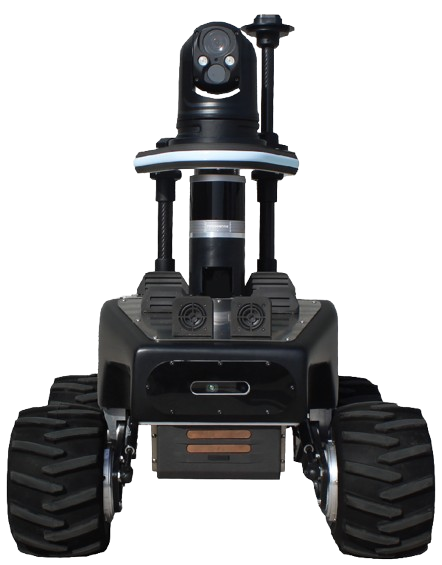
\includegraphics[width=\linewidth]{figures/robotnik_rb_summit_front.png}
        \caption{Vista frontal}
        \label{fig:summit_a}
    \end{subfigure}
    \hfill
    \begin{subfigure}{0.25\linewidth}
        \centering
        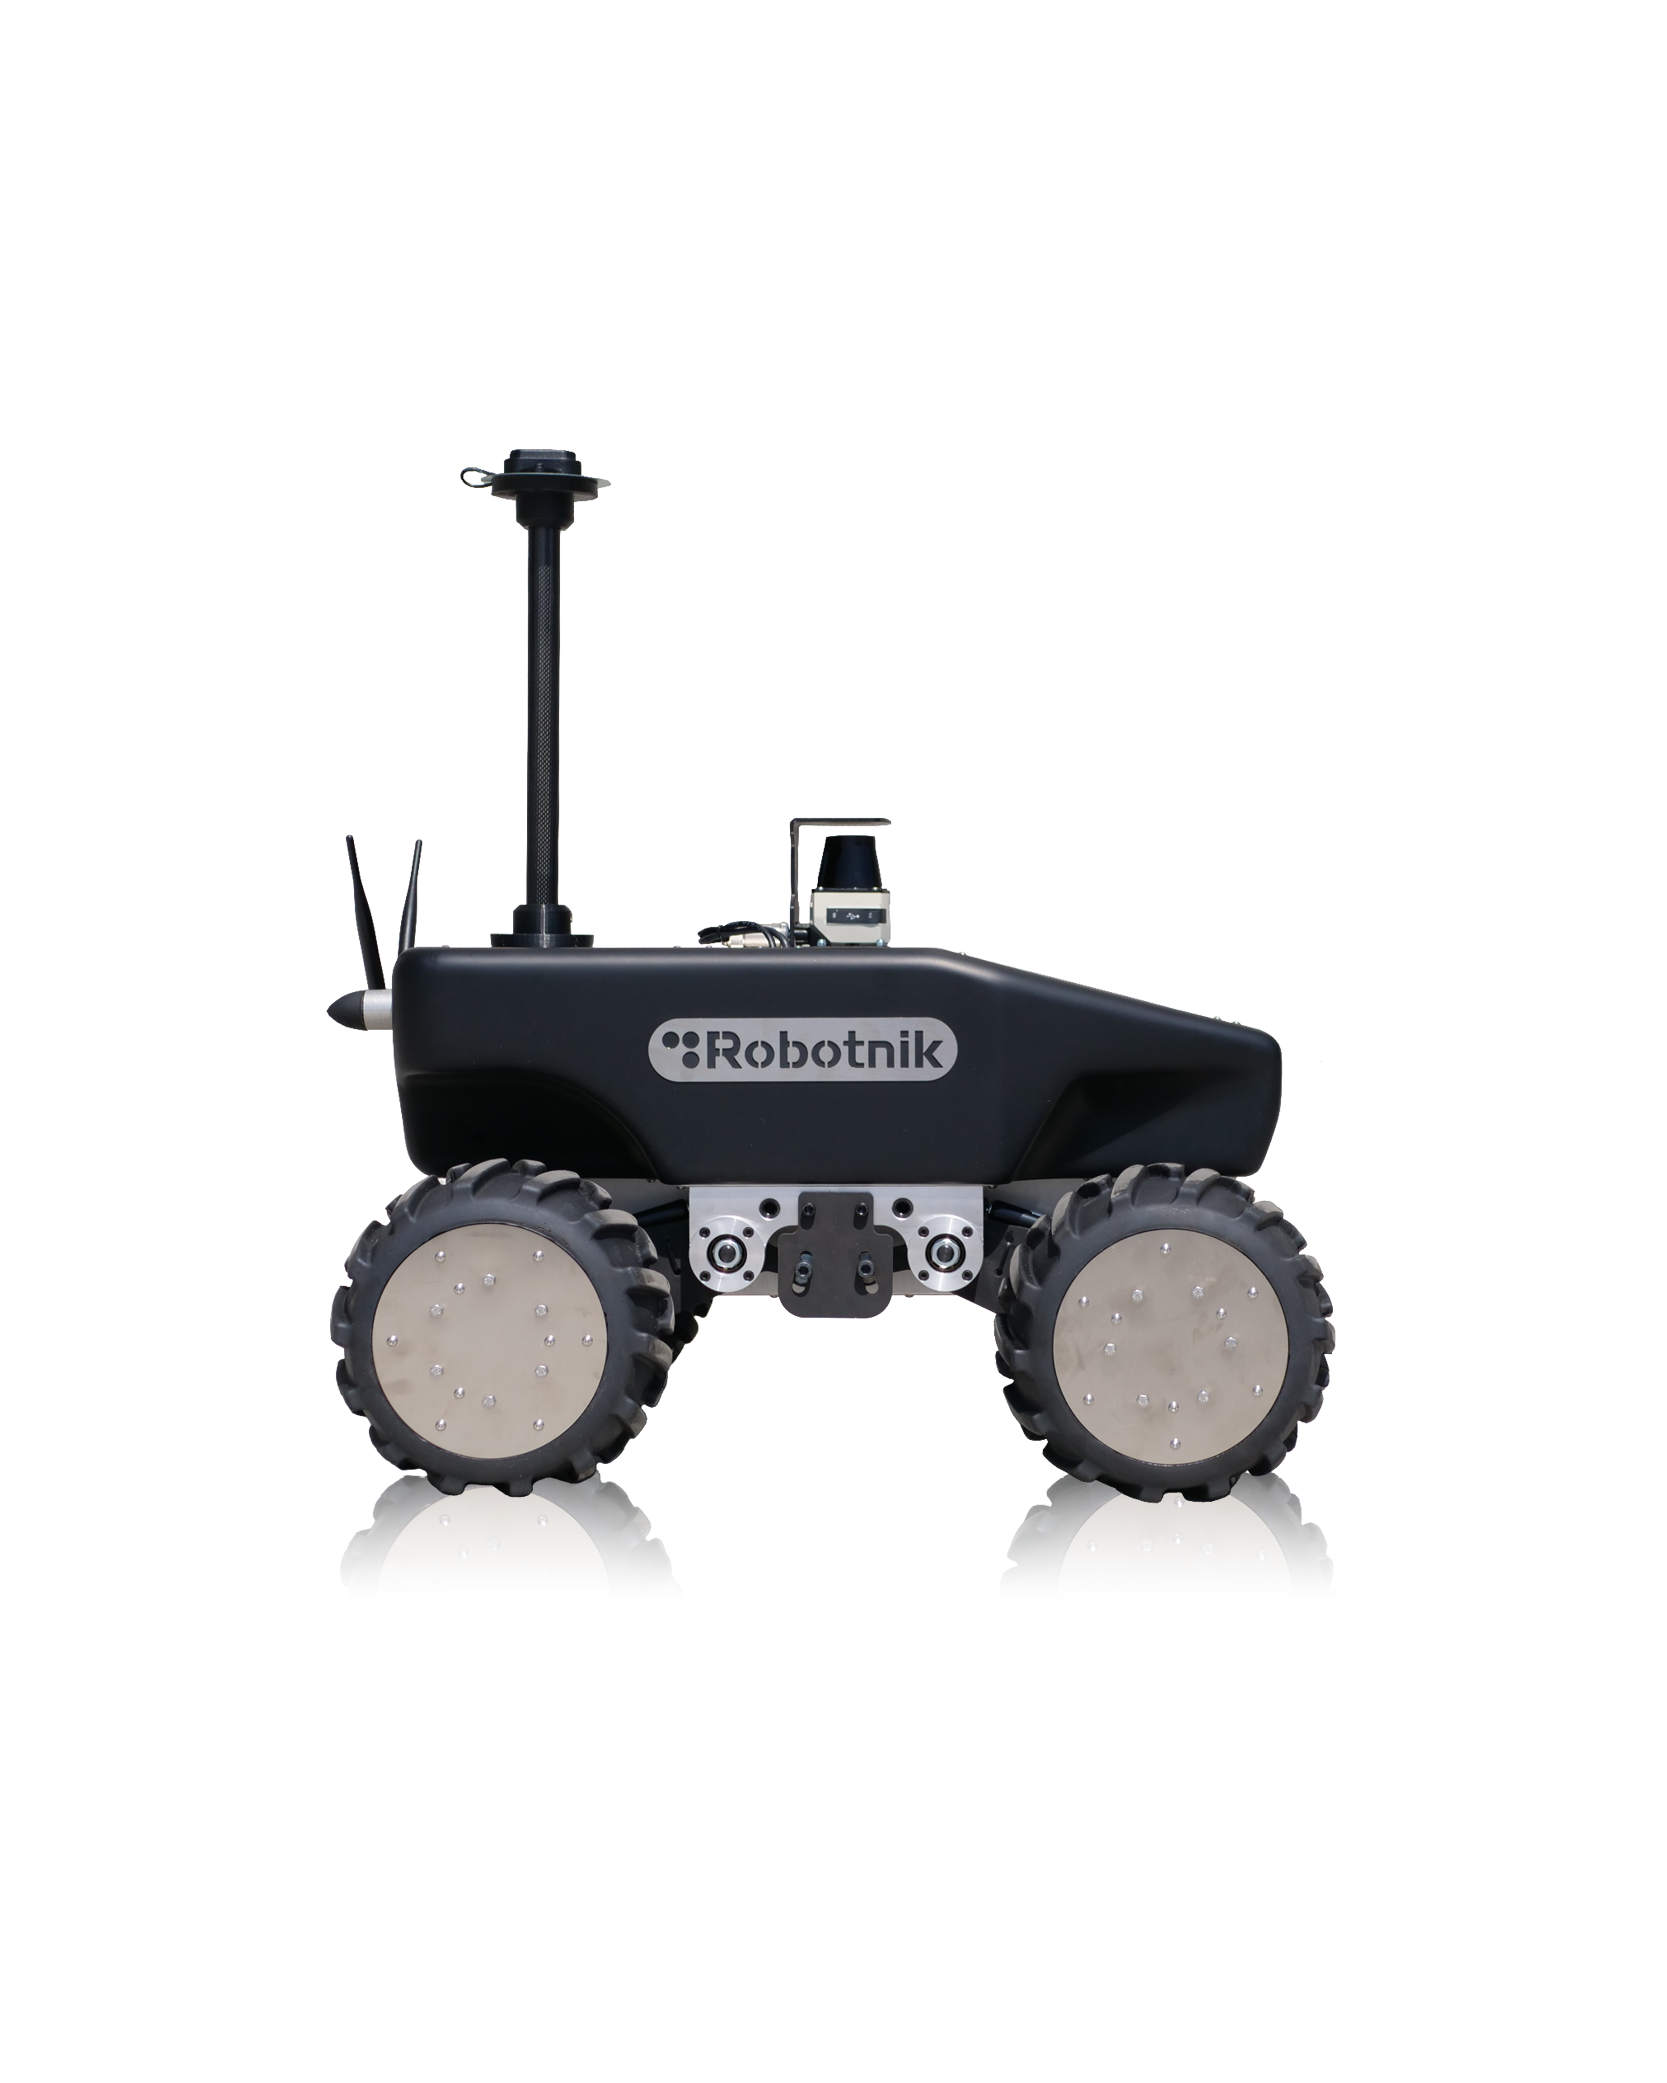
\includegraphics[width=\linewidth]{figures/robotnik_rb_summit_lateral.png}
        \caption{Vista lateral}
        \label{fig:summit_b}
    \end{subfigure}
    \hfill
    \begin{subfigure}{0.25\linewidth}
        \centering
        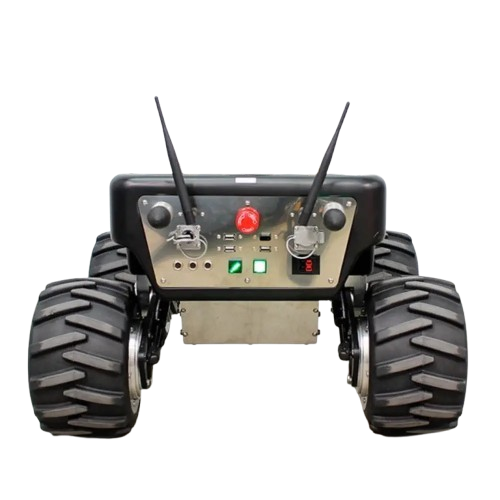
\includegraphics[width=\linewidth]{figures/robotnik_rb_summit_front_back.png}
        \caption{Vista trasera}
        \label{fig:summit_c}
    \end{subfigure}
    \caption{Plataforma Summit XL}
    \label{fig:summit}
\end{figure}

El Summit XL dispone de cuatro ruedas motrices con tracción diferencial tipo \textit{skid-steering}, donde el giro se produce mediante deslizamiento controlado provocado por la diferencia de velocidad entre los laterales derecho e izquierdo. Tiene una elevada capacidad de tracción y robustez mecánica.

El sistema de tracción está compuesto por:
\begin{itemize}
    \item Cuatro servomotores \textit{brushless} de 500 W.
    \item Encoders integrados para realimentación de velocidad y posición.
    \item Controladores de motor interconectados mediante bus \gls{can}.
\end{itemize}

La plataforma alcanza una velocidad máxima de 3 m/s y puede superar pendientes de hasta el 80\%, lo que la hace adecuada para escenarios exigentes.

Las principales especificaciones físicas del robot se recogen en la Tabla~\ref{tab:especificaciones_summit_xl}.

\begin{table}[H]
    \centering
    \begin{tabular}{|l|c|}
        \hline
        Dimensiones & 720 × 614 × 416 mm \\ \hline
        Peso & 65 kg \\ \hline
        Capacidad de carga & 50 kg \\ \hline
        Protección & IP50 \\ \hline
        Rango de temperatura & -10 °C a +45 °C \\ \hline
    \end{tabular}
    \caption{Especificaciones técnicas principales}
    \label{tab:especificaciones_summit_xl}
\end{table}

El sistema de alimentación se basa en una batería LiFePO$_4$ de 15 Ah a 48 V, proporcionando una autonomía de hasta 10 horas en función del perfil de operación.

La plataforma integra un PC industrial embarcado basado en Linux que actúa como unidad central de procesamiento, coordinando el control de actuadores y la adquisición de datos sensoriales. La arquitectura \textit{software} se basa en \gls{ros1}. La arquitectura basada en nodos permite desacoplar los módulos de percepción, localización, planificación y control, habilitando su ejecución local o su externalización hacia la infraestructura Edge a través de la red \gls{5g} privada.


La comunicación entre el ordenador embarcado y los drivers de motor se realiza a través del bus \gls{can}, lo que garantiza comunicación determinista y baja latencia en el control de actuadores.

En términos de conectividad, la plataforma dispone de:
\begin{itemize}
    \item WiFi 802.11n (WiFi-4).
    \item Conectividad interna: USB, RS232 y GPIO.
    \item Conectividad externa: USB, RJ45 y 12 VDC.
\end{itemize}

Estas interfaces permiten la integración directa con la infraestructura de red \gls{5g} privada, descrita en la sección \ref{sec:capa_de_red_5g_privada}, facilitando la transmisión de datos de percepción y control hacia nodos \textit{Edge} distribuidos.

La plataforma admite la integración de distintos sensores en función del caso de uso. En la configuración empleada en este trabajo se consideran:
\begin{itemize}
    \item Unidad de medición inercial (IMU).
    \item Cámara \gls{ptz} para transmisión de vídeo en tiempo real.
    \item Sensor \gls{lidar} para percepción del entorno.
\end{itemize}

De este modo, la plataforma robótica constituye el origen de los flujos de datos de percepción y control que serán procesados localmente o externalizados según la estrategia de \textit{offloading} definida en la arquitectura global del sistema, integrando la capa física con la infraestructura de computación distribuida descrita en capítulos anteriores.
% \subsubsection{Arquitectura Software ROS 1}
% ============================== 3.3. CAPA DE RED 5G PRIVADA ==============================
\subsection{Capa de red 5G privada}
\label{sec:capa_de_red_5g_privada}

La capa de red privada constituye la columna vertebral del entorno experimental, proporcionando conectividad inalámbrica de baja latencia, alto ancho de banda y capacidades avanzadas de segmentación. Esta infraestructura se basa en la red privada 5G desplegada en la \gls{upv}, concebida como entorno de experimentación para aplicaciones avanzadas de \textit{Edge Computing}, \textit{Digital Twins} e \gls{iot} \cite{CrespoAguado2024IoTEdgeCloud} \cite{ITEAM2025Private5G}.

El diseño de esta capa no se limita a ofrecer conectividad radio, sino que integra capacidades de computación en \textit{edge}, virtualización de funciones de red y mecanismos de orquestación inteligente, alineándose con la evolución hacia arquitecturas \gls{5ga} \cite{CrespoAguado2024IoTEdgeCloud}


\subsubsection{Arquitectura general de la red privada}

La red privada \gls{5g} del \gls{iteamupv} constituye la infraestructura de comunicaciones sobre la que se soporta la capa robótica descrita en la Sección \ref{sec:capa_robotica}. Esta red presenta una arquitectura completa en modo \gls{5gsa}, con despliegue \textit{indoor} y \textit{outdoor}, múltiples bandas de frecuencia y diversas implementaciones de núcleo \gls{5g} \cite{ITEAM2025Private5G}.

Desde el punto de vista funcional, la arquitectura se estructura en cuatro bloques principales:

\begin{enumerate}
    \item \textbf{Radio Access Network (RAN)}

    La \gls{ran} es el subsistema encargado de proporcionar conectividad radio entre los \gls{ues} y el núcleo \gls{5g}. Entre las características más relevantes del equipamiento empleado destacan:

    \begin{itemize}
        \item Ancho de banda de hasta 100 MHz.
        \item Configuración flexible en \textit{Time Division Duplex} (TDD).
        \item Soporte MIMO 4x4.
        \item Arquitectura funcionalmente separada \gls{cu_du_ru}.
    \end{itemize}

    La separación funcional \gls{cu_du_ru} permite desacoplar el procesamiento de la capa física de las capas superiores, reducir la latencia situando la \gls{du} próxima a la unidad radio y virtualizar la \gls{cu} sobre infraestructura de propósito general. Asimismo, el soporte de \textit{radio slicing} mediante asignación dinámica de recursos físicos (PRBs) permite priorizar determinados flujos de tráfico en función de los requisitos de cada aplicación.

    En aplicaciones de robótica móvil, la \gls{ran} resulta crítica al garantizar un \textit{uplink} robusto para la transmisión de datos sensoriales y minimizar el \textit{jitter} en escenarios de teleoperación.

    \item \textbf{Núcleo \gls{5g} (\gls{5g} Core)}

    El núcleo \gls{5g} implementa las funciones del plano de control (\textit{Control Plane}) y del plano de usuario (\textit{User Plane}). El núcleo sigue una arquitectura \gls{sba}, propia de \gls{5gsa}, lo que permite la virtualización y desacoplamiento de funciones de red sobre infraestructura de propósito general.

    Estas funciones pueden ejecutarse de forma virtualizada tanto en infraestructura \textit{Edge} como en \textit{Cloud}, tal y como se representa en la Figura~\ref{fig:arquitectura_5Gsa}.

    La posibilidad de instanciar múltiples \gls{upf} habilita mecanismos de \textit{network slicing} a nivel de \textit{core}, permitiendo:

    \begin{itemize}
        \item Aislar tráfico por aplicación.
        \item Implementar políticas de QoS diferenciadas.
        \item Aproximar el plano de usuario al \textit{Edge}.
    \end{itemize}

    En sistemas distribuidos basados en \gls{ros} con estrategias de \textit{offloading}, la proximidad de la \gls{upf} a los nodos \textit{Edge} reduce la latencia \gls{e2e} en la transmisión de \textit{topics} de alta tasa, lo que resulta determinante en aplicaciones sensibles al retardo.

    \item \textbf{Infraestructura Edge asociada al plano de usuario}

    La infraestructura \textit{Edge} constituye el punto intermedio del \textit{continuum} 	\textit{Robot--Edge--Cloud} \cite{CrespoAguado2024IoTEdgeCloud}. Asociada al plano de usuario, permite ejecutar tareas de procesamiento con requisitos estrictos de latencia.

    La infraestructura \textit{edge} puede alojar instancias virtualizadas de la \gls{upf}, aproximando el plano de usuario a los dispositivos finales y reduciendo la latencia \gls{e2e}. Esta integración refuerza el carácter distribuido y programable de la arquitectura, alineado con el paradigma de \gls{nfv}.

    En el contexto de robótica móvil, el \textit{edge} posibilita:

    \begin{itemize}
        \item Teleoperación inmersiva.
        \item Procesamiento en tiempo real de vídeo.
        \item \textit{Offloading} de algoritmos de \gls{slam} de elevada complejidad computacional.
        \item Inferencia de modelos de inteligencia artificial.
    \end{itemize}

    Este enfoque reduce la carga computacional del robot y evita el envío continuo de grandes volúmenes de datos al \textit{cloud}.

    \item \textbf{Interconexión con cloud}

    La interconexión con infraestructuras \textit{cloud} permite ejecutar tareas computacionalmente intensivas no críticas en latencia, tales como:

    \begin{itemize}
        \item Procesamiento Big Data.
        \item Entrenamiento de modelos de aprendizaje automático.
        \item Almacenamiento histórico de datos.
    \end{itemize}

    Este diseño desacopla los procesos sensibles a la latencia (gestionados en \textit{edge}) de aquellos con mayores requerimientos computacionales pero menor criticidad temporal (gestionados por el \textit{cloud}) \cite{ITEAM2025Private5G}.
\end{enumerate}

Como se muestra en la Figura~\ref{fig:arquitectura_5Gsa}, la arquitectura integra la red privada \gls{5g} con la infraestructura \textit{edge} y la interconexión \textit{cloud} bajo un esquema de orquestación dual (\textit{Network Orchestration} y \textit{Edge Orchestration}). Esta separación permite la gestión dinámica de recursos, la instanciación de funciones de red virtualizadas y el despliegue automatizado de aplicaciones distribuidas.

\begin{figure}[H]
    \centering
    \includegraphics[width=0.85\linewidth]{figures/arquitectura_5Gsa.png}
    \caption{Arquitectura funcional de la red privada \gls{5gsa} integrada con infraestructura \textit{Edge} y \textit{Cloud}, donde se muestra la virtualización de funciones de red y aplicaciones, así como los mecanismos de orquestación \cite{ITEAM2025Private5G}.}
    \label{fig:arquitectura_5Gsa}
\end{figure}

La adopción de una red privada \gls{5g} como capa de red del sistema experimental responde a la necesidad de garantizar aislamiento lógico, control determinista de \gls{qos} y segmentación mediante \textit{network slicing}, capacidades que no están disponibles de forma nativa en tecnologías inalámbricas convencionales como IEEE 802.11 (WiFi), especialmente en entornos con tráfico heterogéneo y requisitos de baja latencia.

Desde una perspectiva sistémica, la red privada no actúa únicamente como medio de transporte de datos, sino como un componente activo del sistema distribuido, alineado con el paradigma 	\textit{Robot--Edge--Cloud} y con los requisitos de aplicaciones avanzadas como Digital Twins y teleoperación inmersiva.

% Finalmente, la red privada opera en las bandas n40 y n78, lo que permite evaluar compromisos entre cobertura, capacidad y latencia.
% ============================== 3.4. CAPA EDGE ==============================
% \input{sections/03_arquitectura_del_sistema_propuesto/03_04_capa_edge/03_04_00_capa_edge}
% ============================== 3.5. FLUJO DE EXTREMO A EXTREMO ==============================
% \subsection{Flujo de extremo a extremo}
% ================================================================
% 04. ARQUITECTURA EXPERIMENTAL
% ================================================================

% ================================================================
% 05. ANALISIS DE LATENCIA DEL SISTEMA
% ================================================================
\section{Análisis de latencia del sistema}
\subsection{Análisis de latencia del sistema centralizado}

\subsubsection{Procesamiento y modelado de los datos}

El análisis de latencias se ha realizado mediante la 
construcción de un modelo secuencial del sistema, 
representado como un pipeline de eventos: 
\textit{Decisión $\rightarrow$ 
Arbitraje $\rightarrow$ Ejecución $\rightarrow$ Percepción}. 
Este modelo permite descomponer la latencia end-to-end 
en contribuciones parciales por subsistema.

\begin{figure}[h]
    \centering
    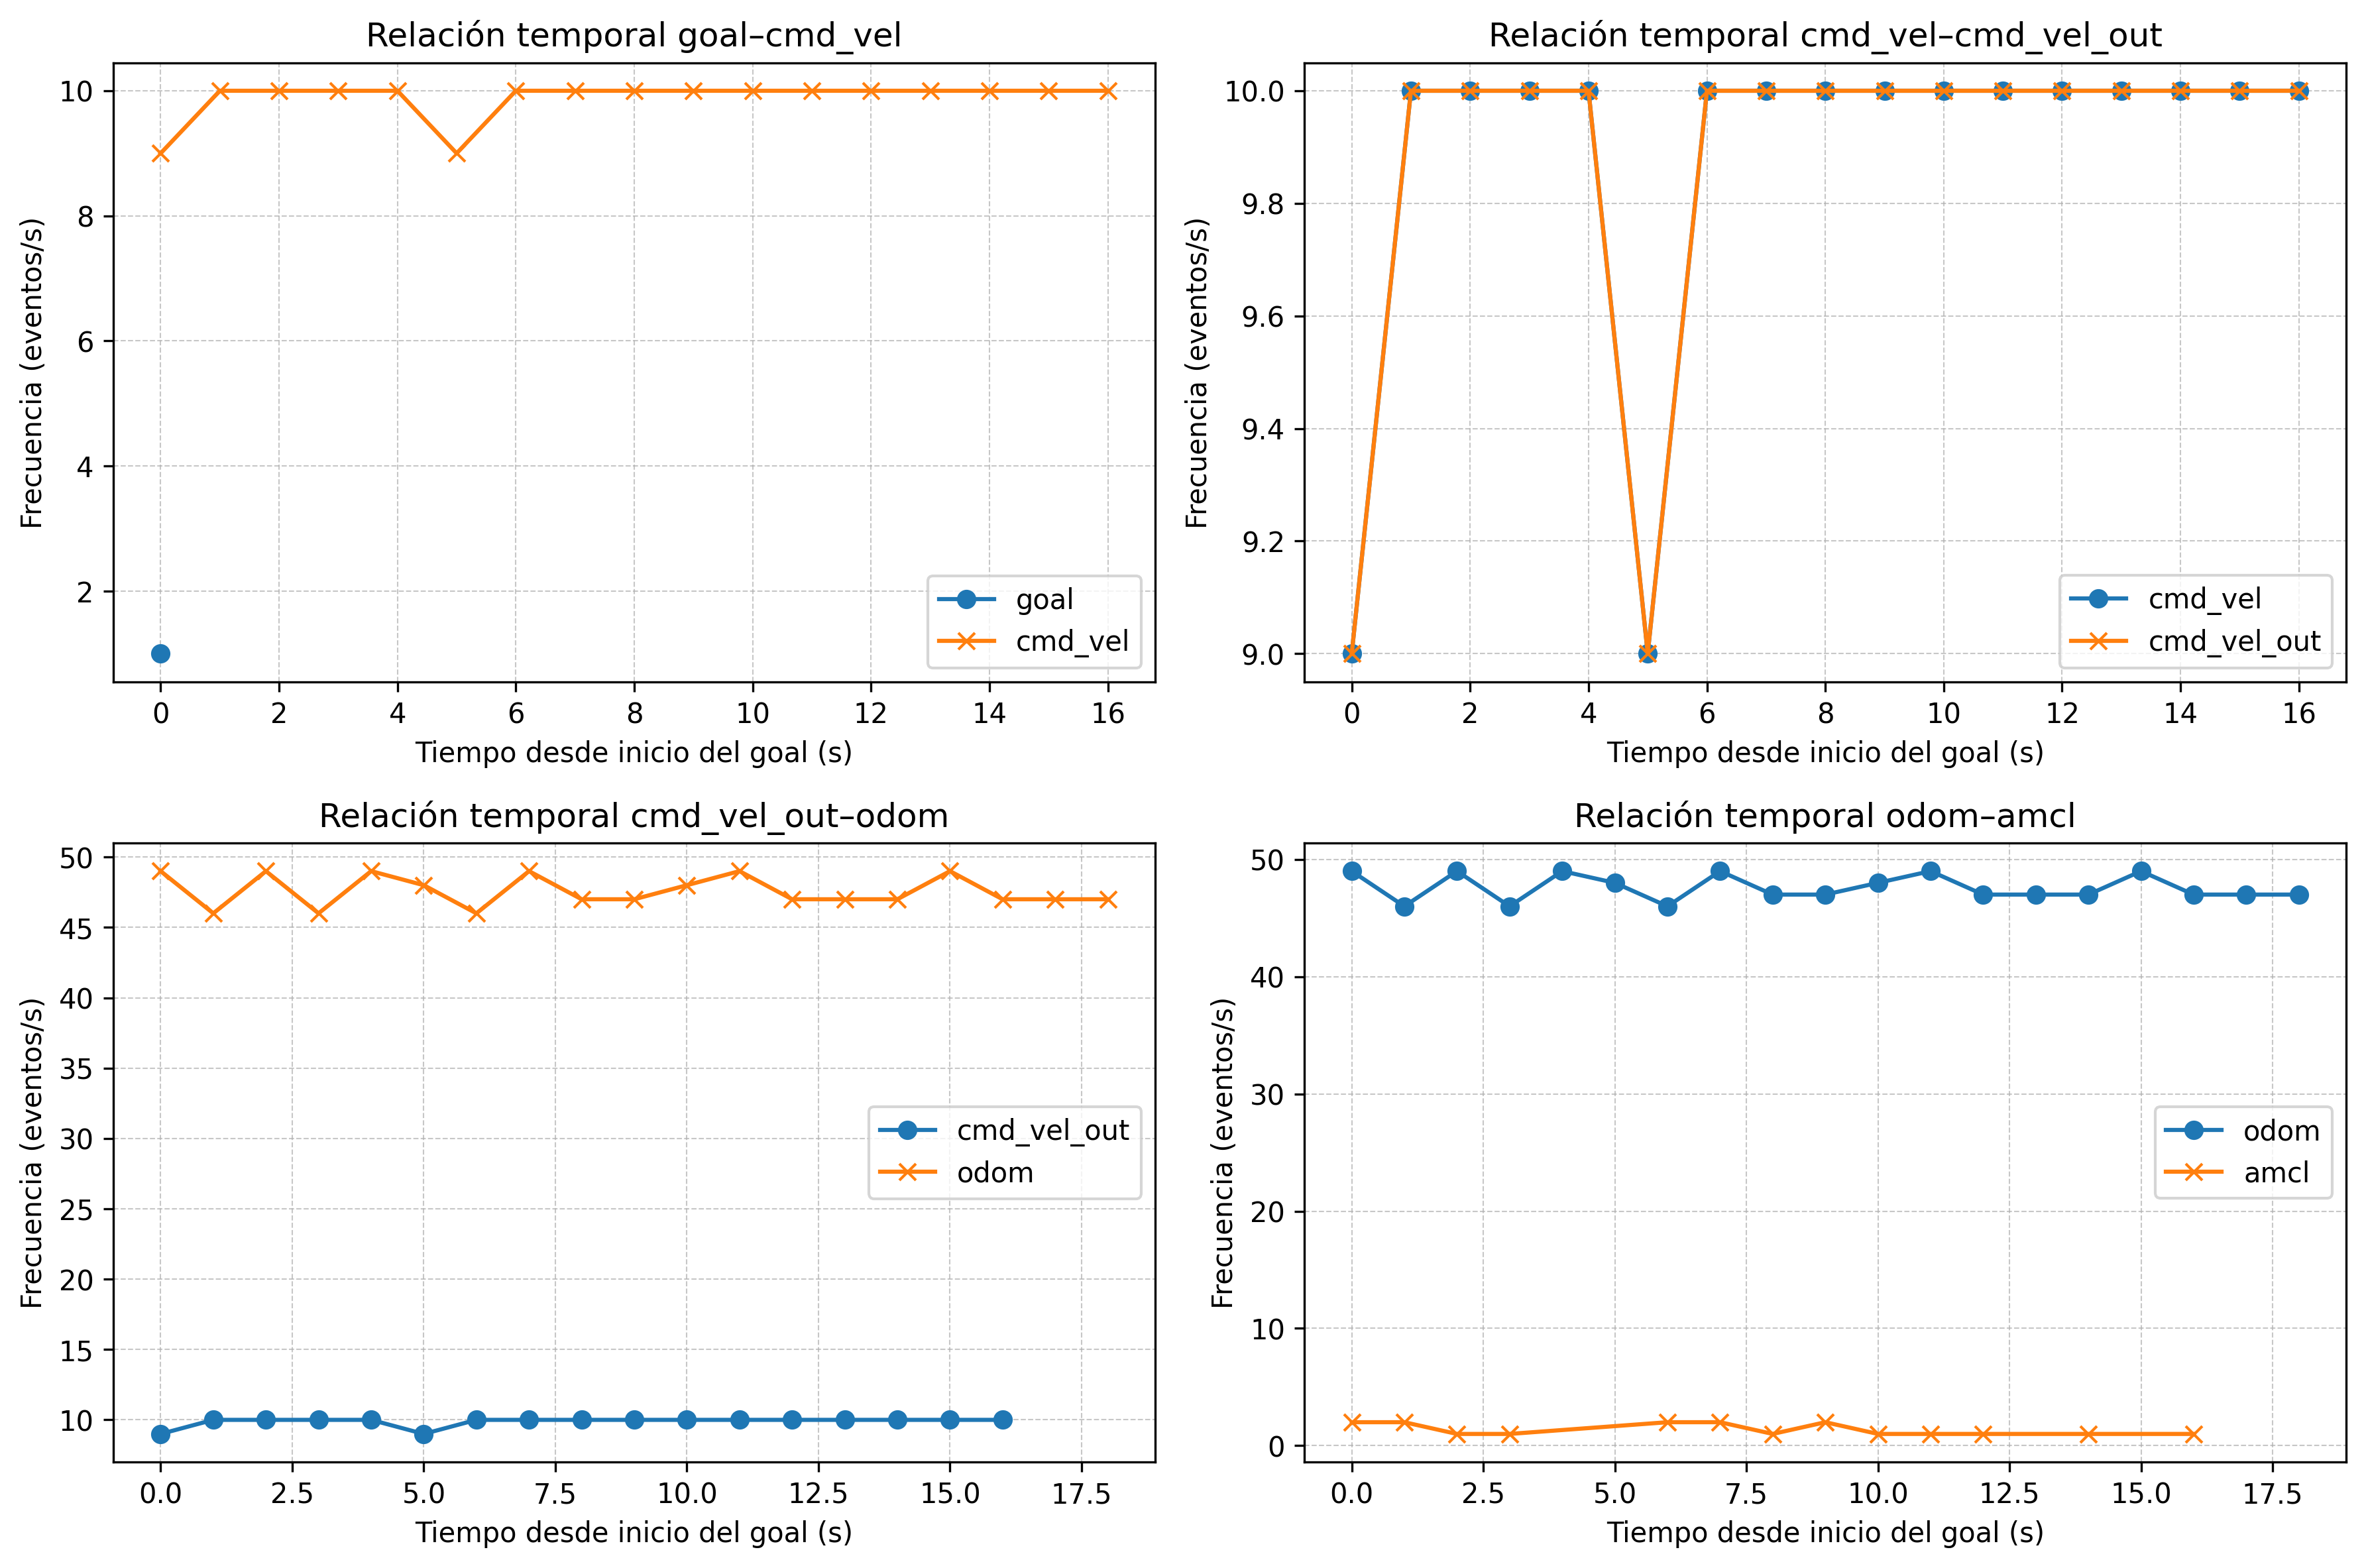
\includegraphics[width=0.9\linewidth]{figures/asynchronous_event_frequencies.png}
    \caption{Frecuencia de publicación de los distintos subsistemas a lo largo del tiempo para un objetivo representativo.}
    \label{fig:asynchronous_event_frequencies}
\end{figure}

No obstante, esta representación constituye una simplificación 
del comportamiento real del sistema. En la práctica, los distintos 
subsistemas operan de forma parcialmente desacoplada, con dependencias 
que se aproximan mejor a una estructura de grafo acíclico dirigido (DAG), 
donde múltiples flujos de información evolucionan de manera asíncrona. 
La interpretación como un modelo lineal event-driven se adopta, por tanto, 
como una aproximación práctica que permite estructurar el análisis, 
asumiendo una relación causal dominante entre eventos.

Esta asincronía se pone de manifiesto en la Figura \ref{fig:asynchronous_event_frequencies}, 
donde se observa un desacoplamiento en las frecuencias de publicación 
de los distintos subsistemas, especialmente en los tramos 
\textit{cmd\_vel\_out--odom} y \textit{odom--amcl}, donde existen relaciones de tipo uno-a-muchos y muchos-a-uno. 
Este comportamiento evidencia la naturaleza asíncrona del sistema. Como consecuencia, la selección de eventos 
basada en el criterio de primer evento posterior puede no capturar 
adecuadamente la correspondencia temporal entre señales.

Para mitigar este efecto, se aplica un tratamiento selectivo de las series temporales mediante 
\textit{Dynamic Time Warping} (DTW), un algoritmo que mide la similitud entre secuencias permitiendo 
deformaciones no lineales en el eje temporal. Este enfoque resulta especialmente adecuado cuando 
existen discrepancias en la frecuencia de eventos, ya que proporciona una alineación 
temporal más consistente entre subsistemas.
\subsubsection{Resultados del análisis de latencia}

\begin{figure}[ht]
    \centering
    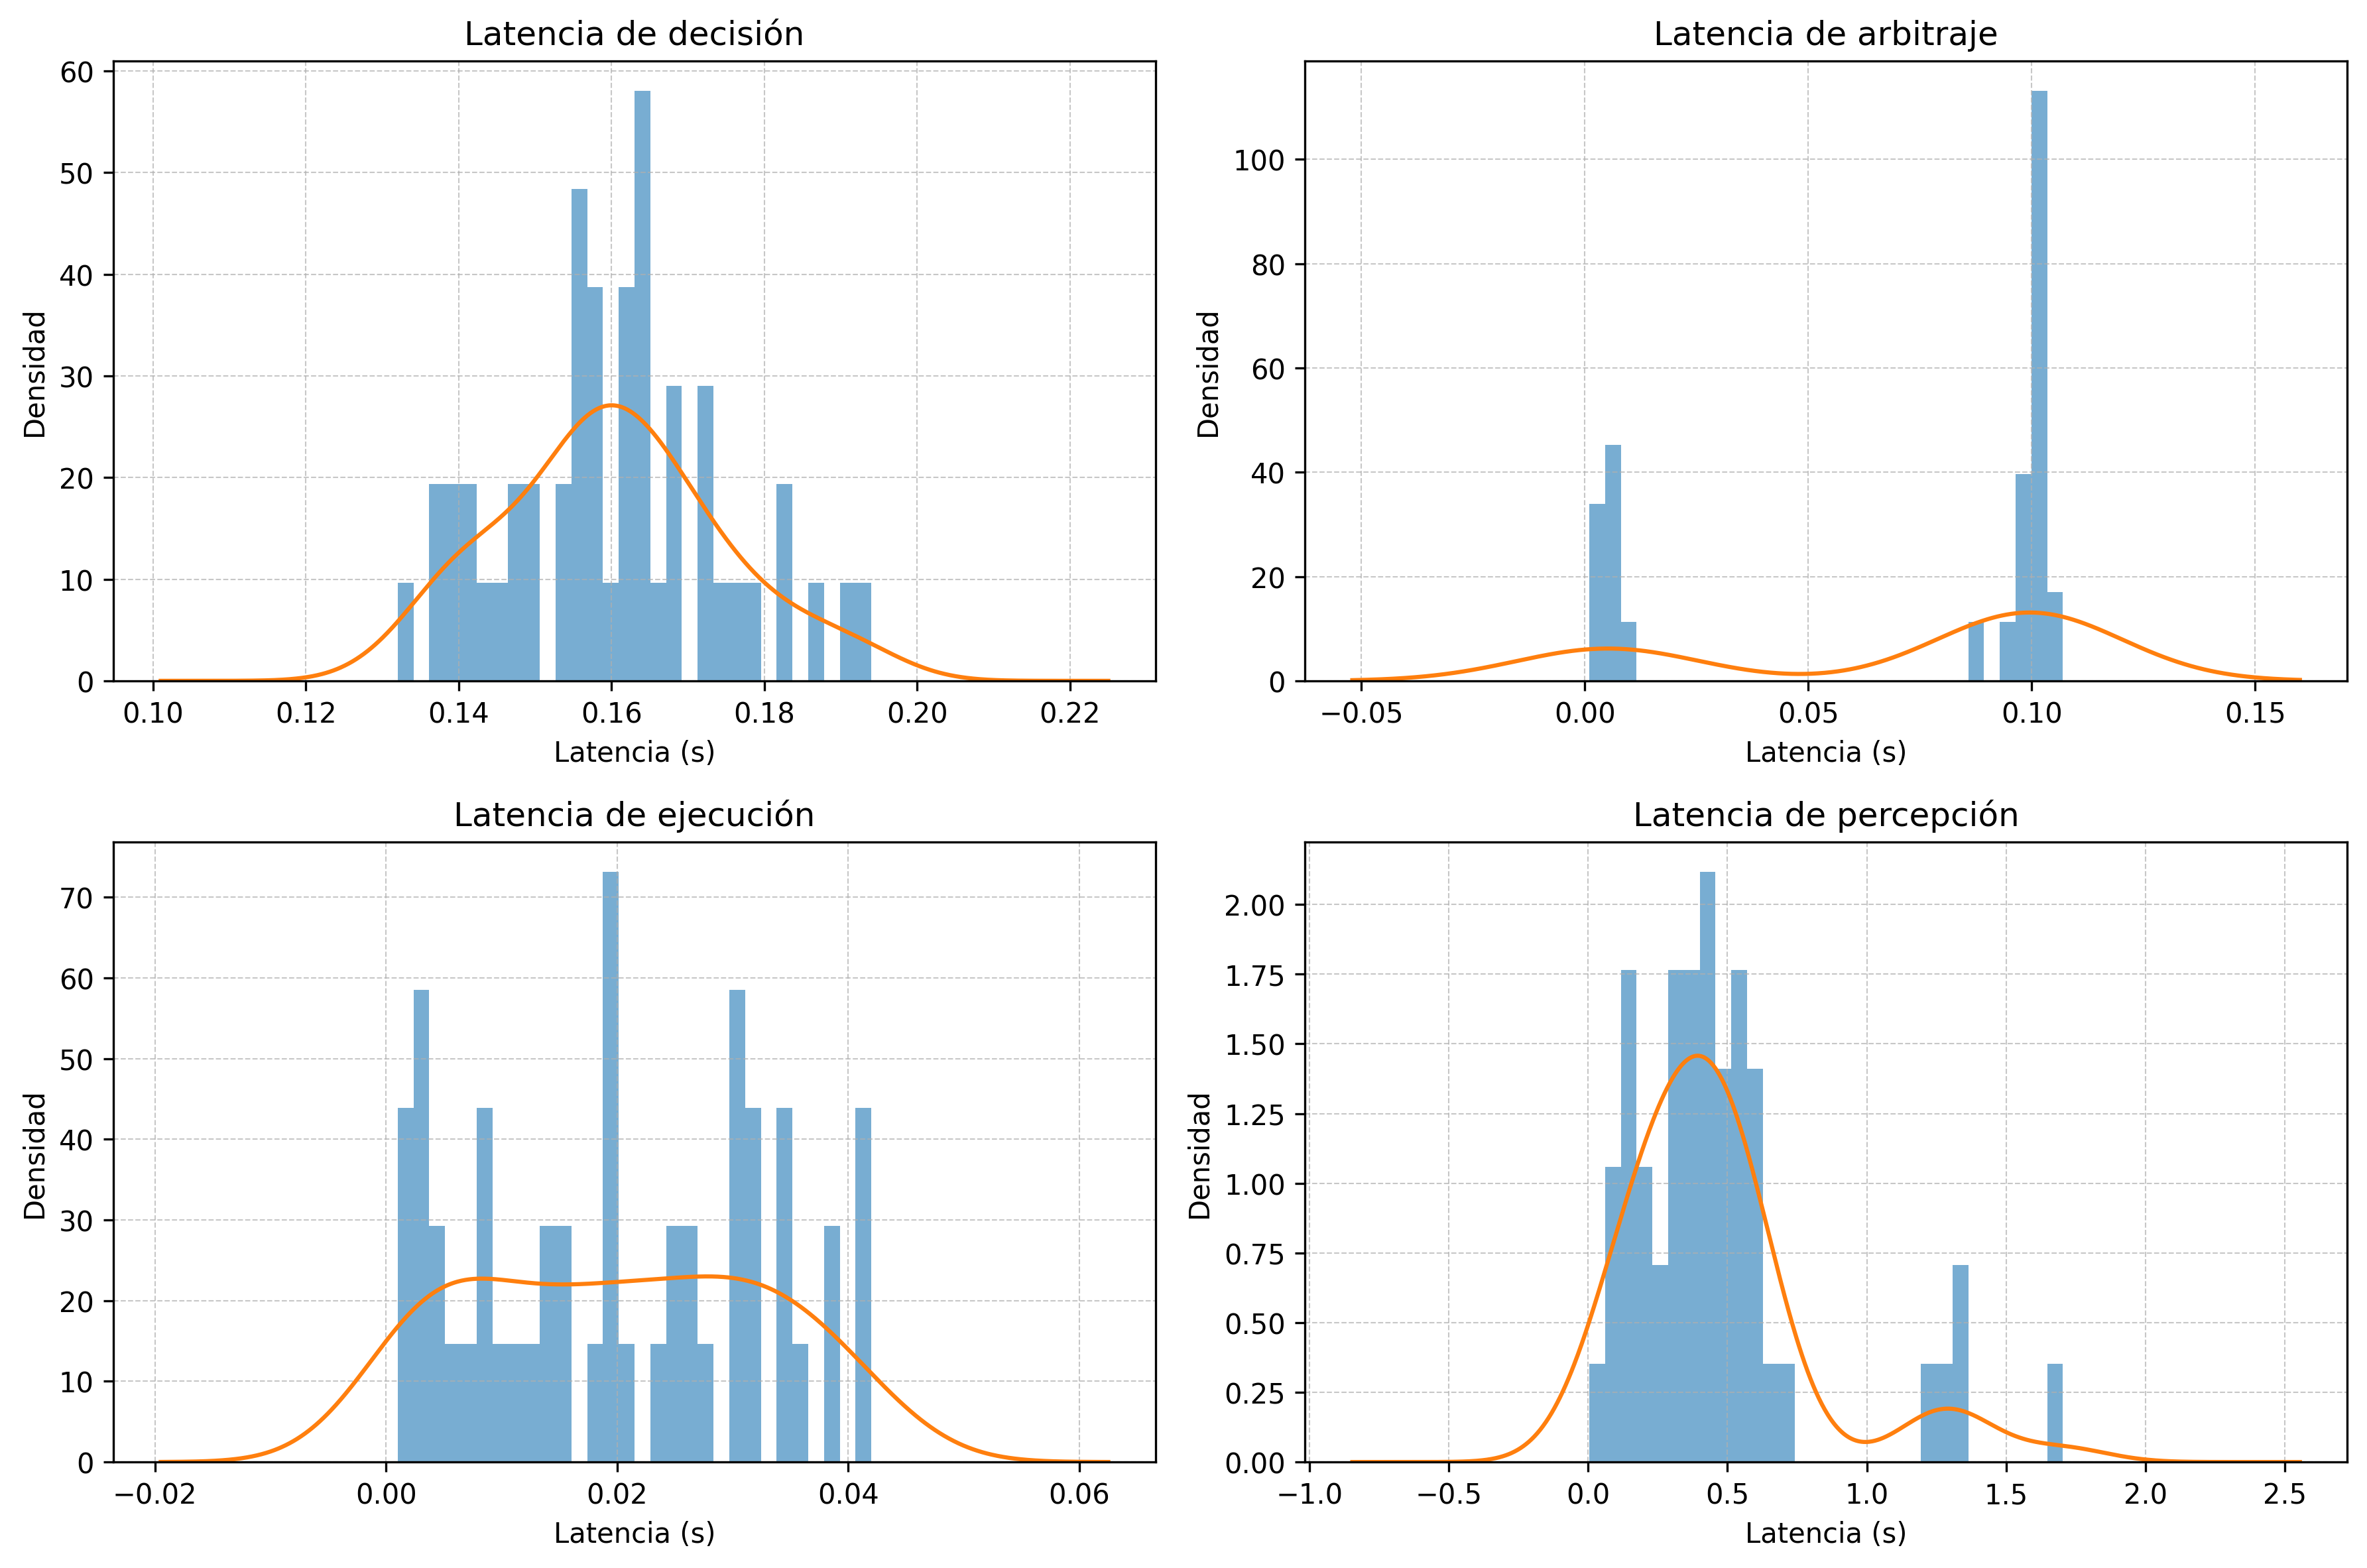
\includegraphics[width=0.9\linewidth]{figures/subsystem_latency_density_distribution.png}
    \caption{Distribución de latencias por subsistema.}
    \label{fig:subsystem_latency_density_distribution}
\end{figure}

\begin{figure}[ht]
    \centering
    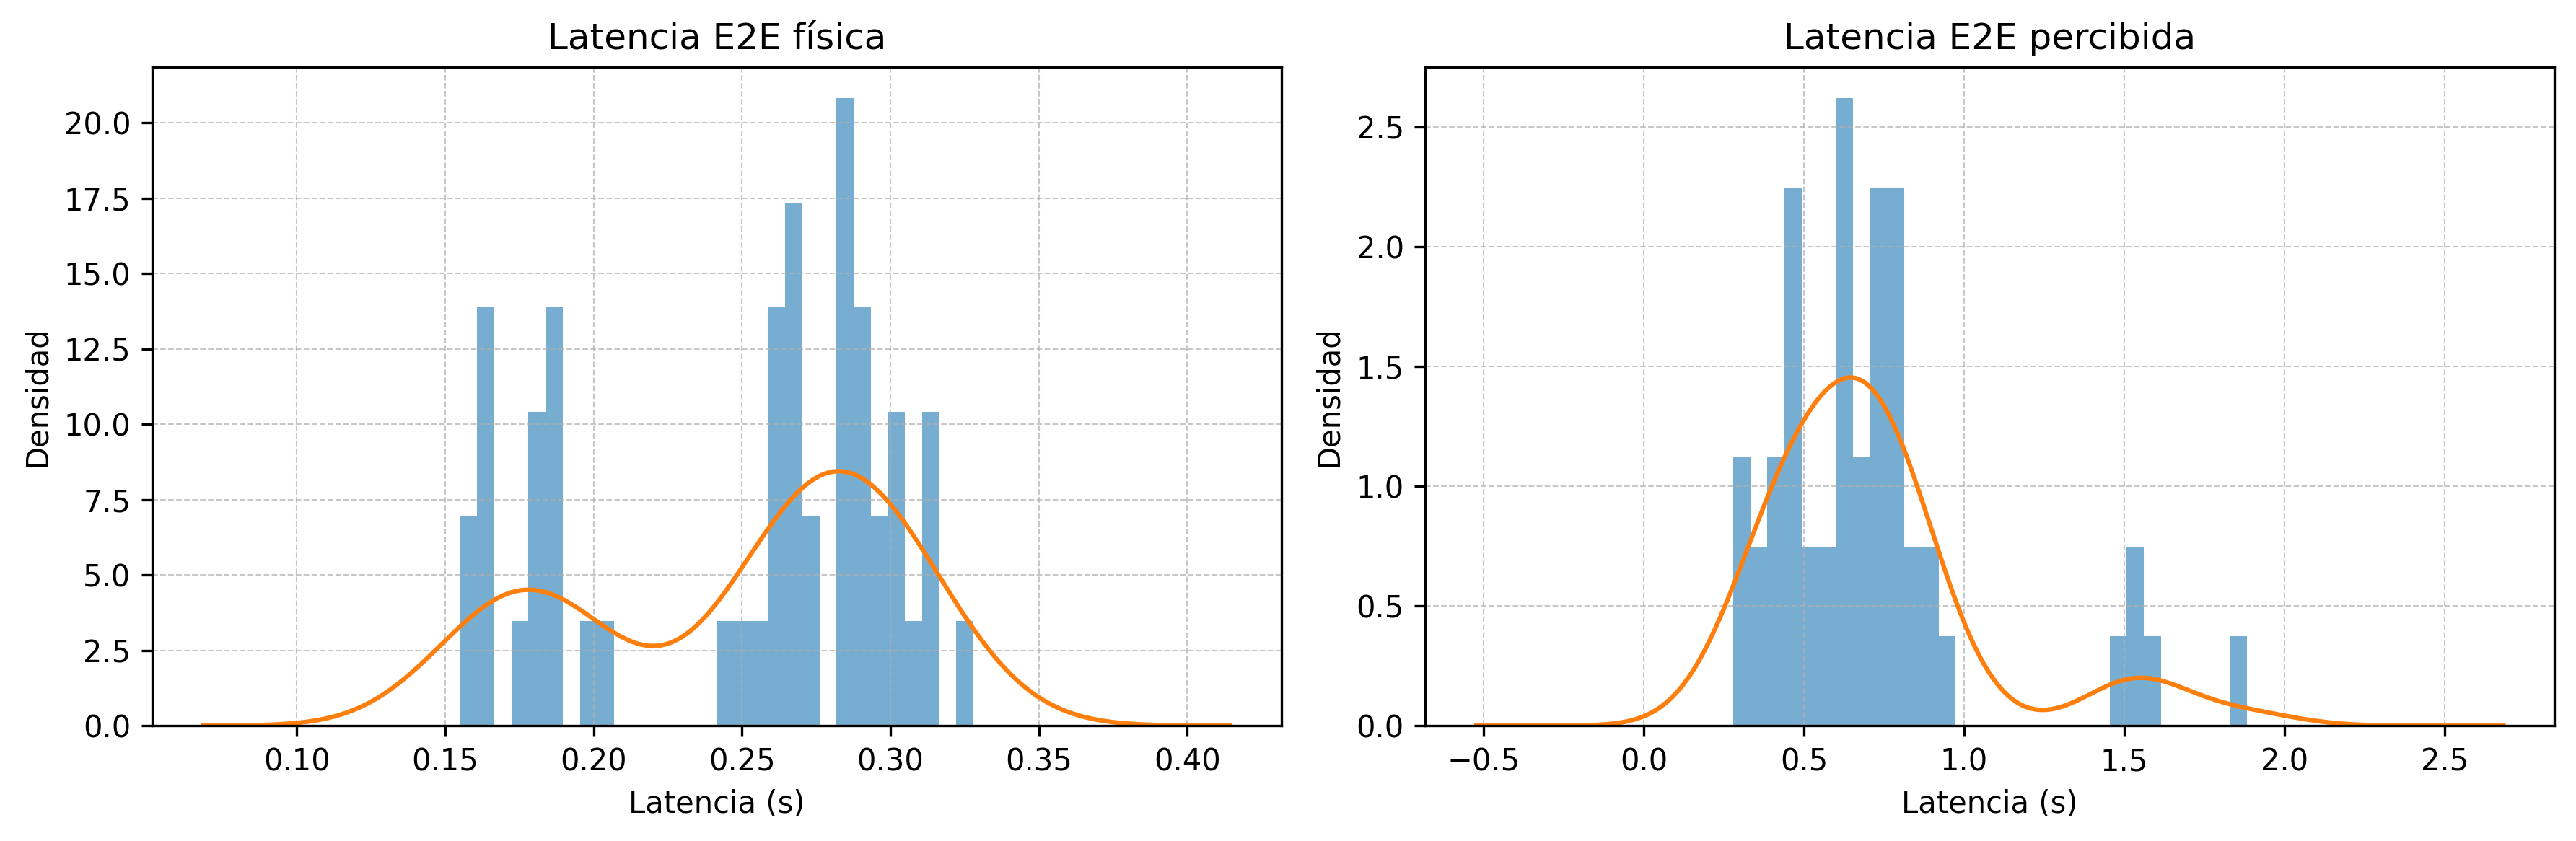
\includegraphics[width=0.9\linewidth]{figures/e2e_latency_density_distribution.png}
    \caption{Distribución de densidad de la latencia end-to-end.}
    \label{fig:e2e_latency_density_distribution}
\end{figure}

\begin{figure}[ht]
    \centering
    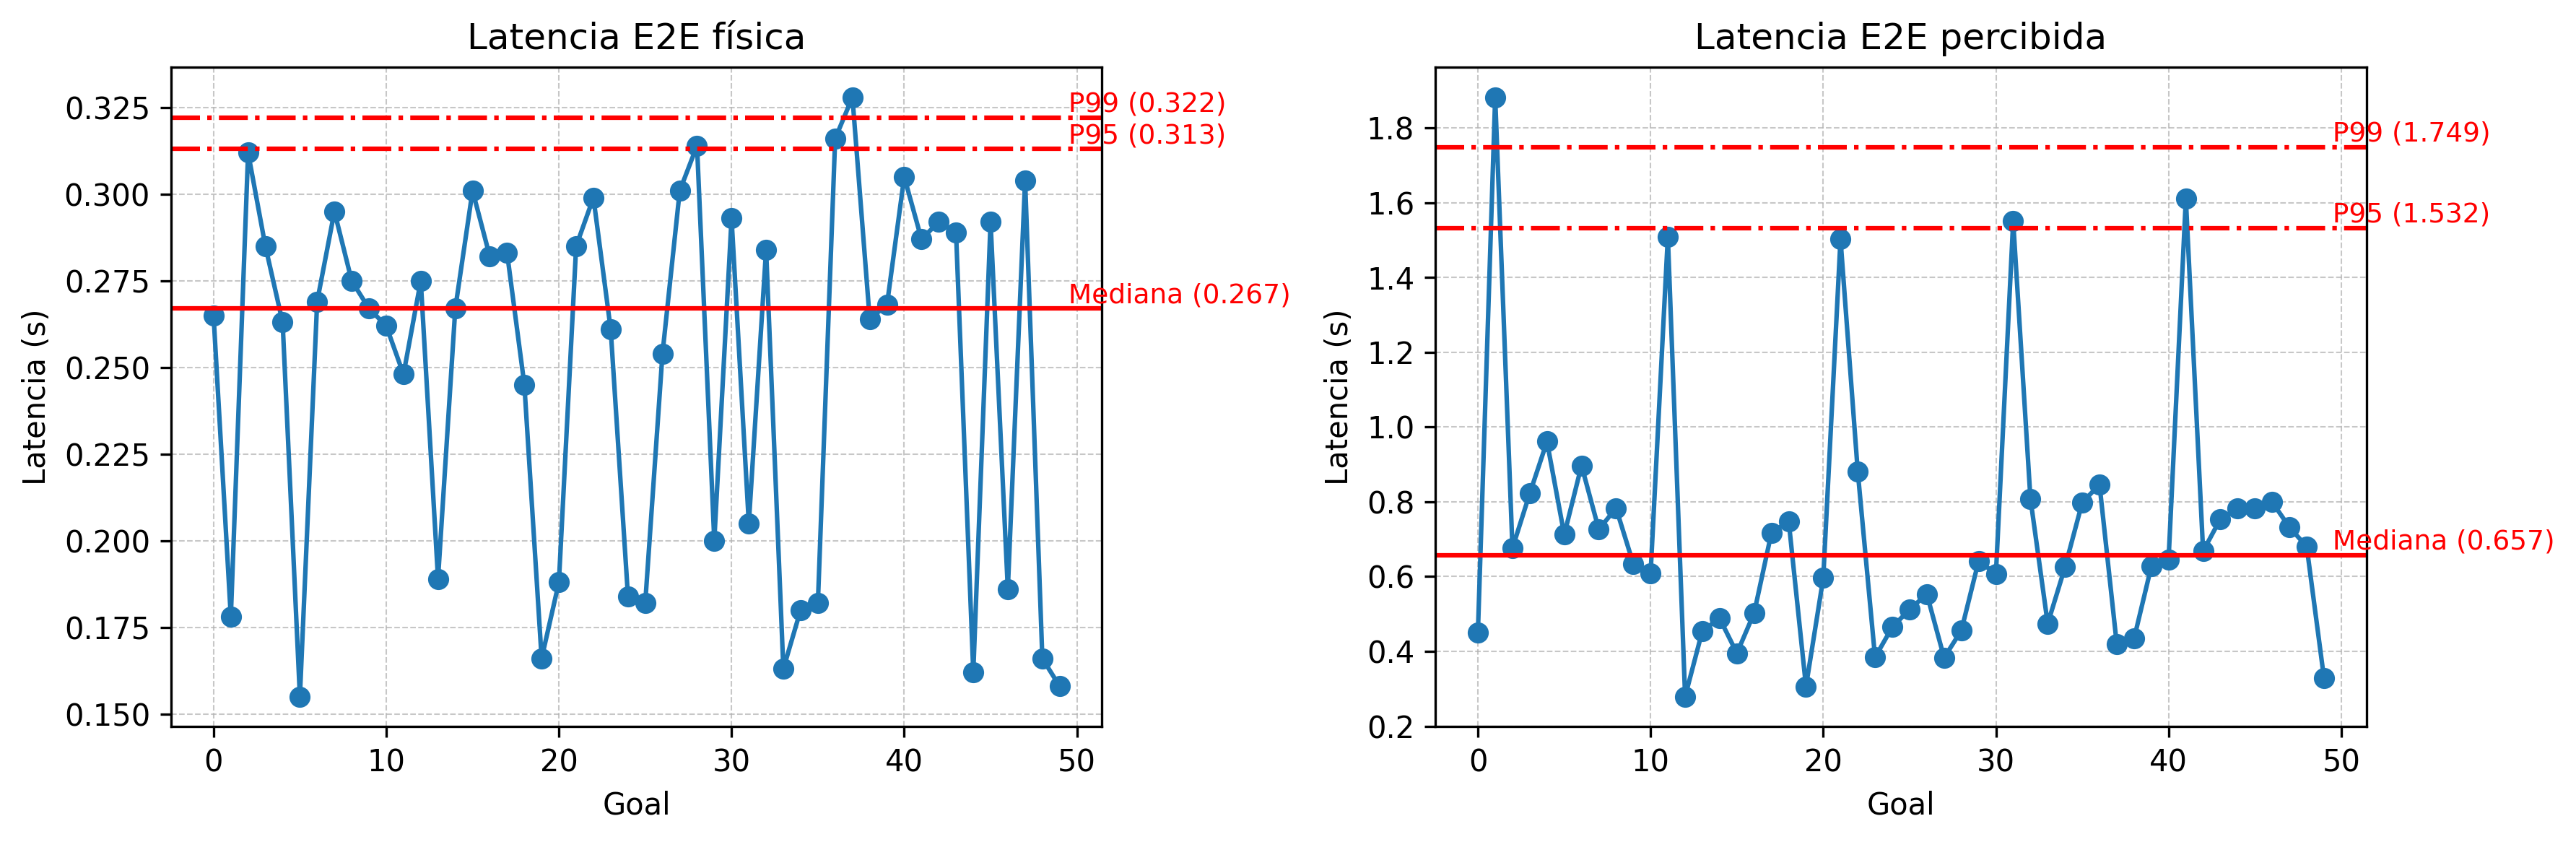
\includegraphics[width=0.9\linewidth]{figures/e2e_latency_per_goal.png}
    \caption{
    Evolución de la latencia end-to-end por objetivo.}
    \label{fig:e2e_latency_per_goal}
\end{figure}


\begin{figure}[ht]
    \centering
    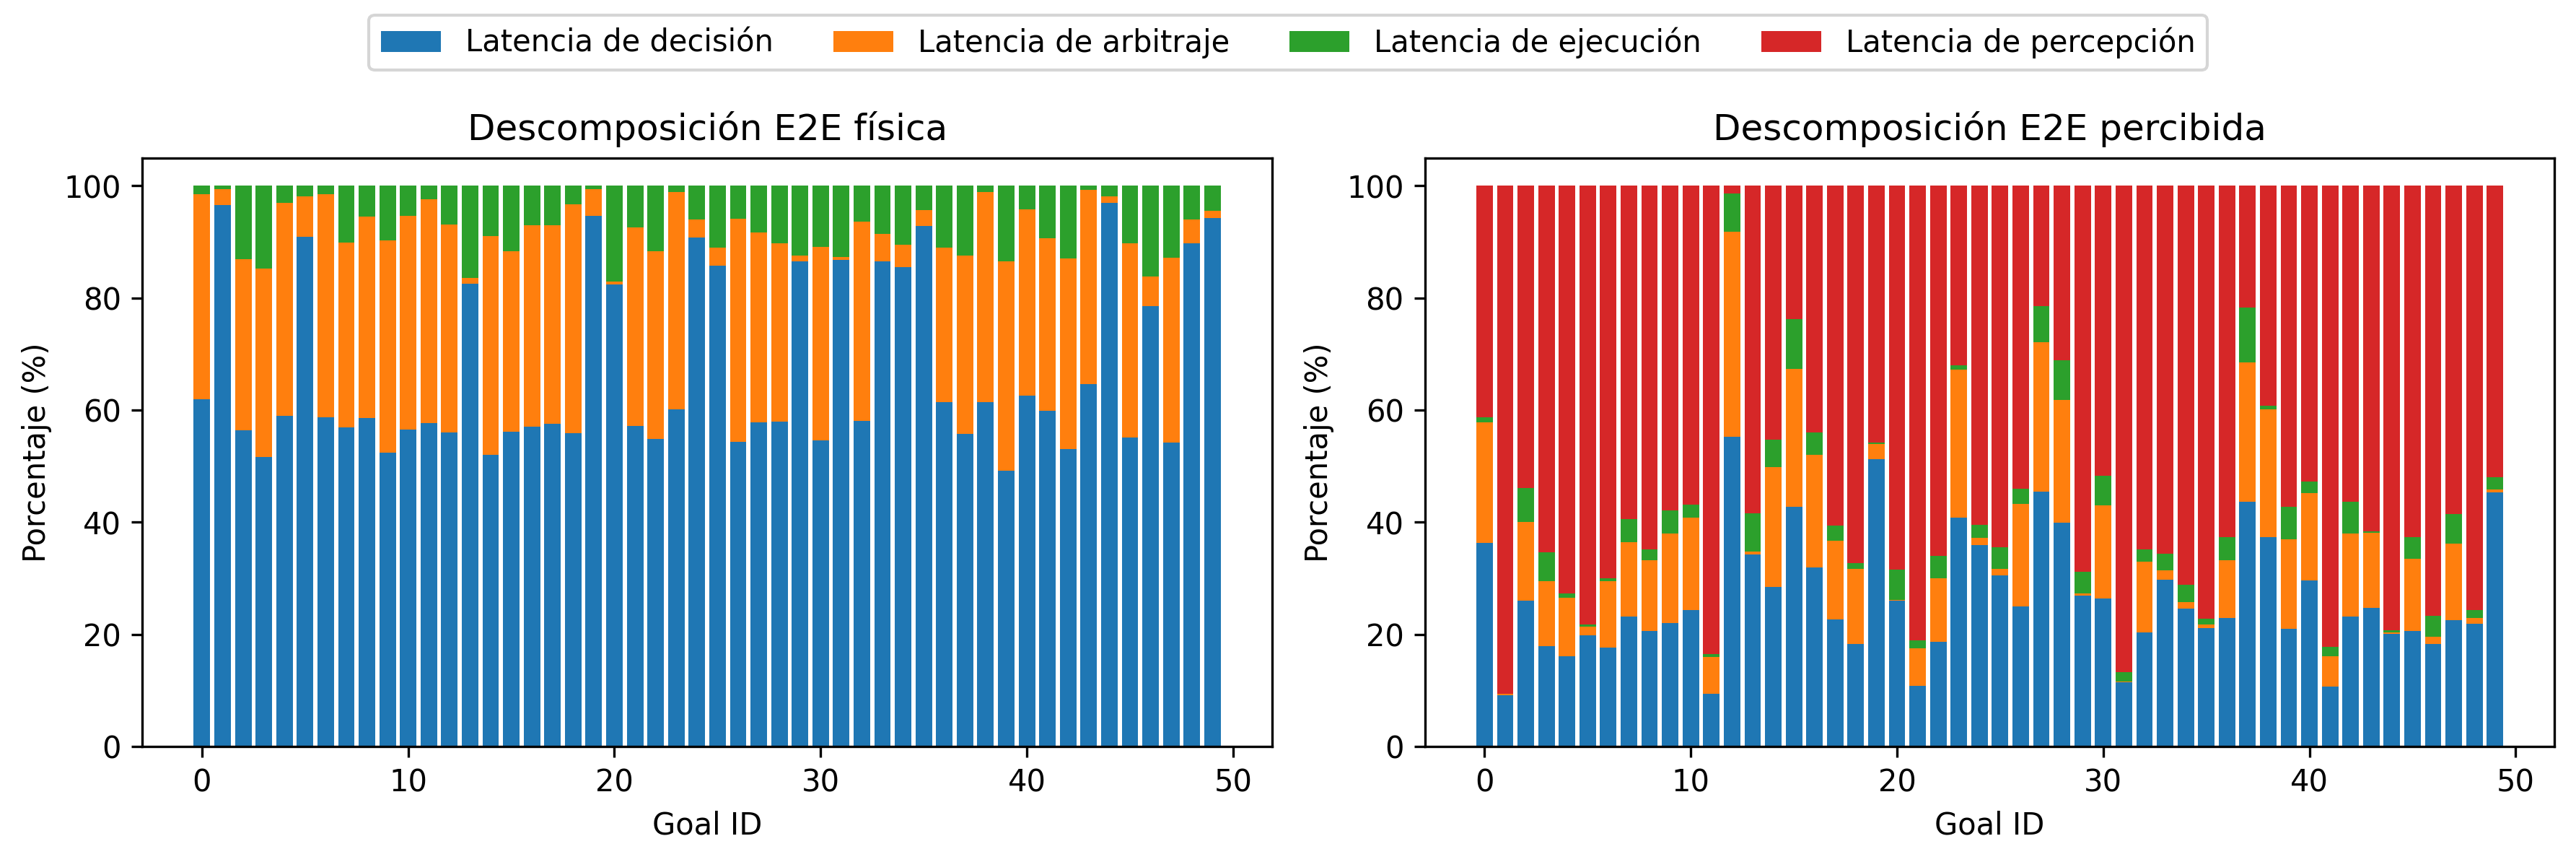
\includegraphics[width=0.9\linewidth]{figures/e2e_latency_decomposition.png}
    \caption{
    Descomposición de la latencia end-to-end de cada objetivo en latencias de los subsistemas.}
    \label{fig:e2e_latency_decomposition}
\end{figure}

\begin{table}[ht]
    \centering
    \small
    \begin{tabular}{lcccccc}
    \hline
    \textbf{Métrica} & \textbf{$L_{decision}$} & \textbf{$L_{arbitraje}$} & \textbf{$L_{ejecucion}$} & \textbf{$L_{percepcion}$} & \textbf{$L_{E2E fisica}$} & \textbf{$L_{E2E percibida}$} \\
    \hline
    Media     & 0.1602 & 0.0693 & 0.0200 & 0.4684 & 0.2495 & 0.7179 \\
    Desv. std & 0.0143 & 0.0446 & 0.0127 & 0.3502 & 0.0531 & 0.3457 \\
    Mínimo    & 0.1320 & 0.0010 & 0.0010 & 0.0040 & 0.1550 & 0.2790 \\
    P50       & 0.1605 & 0.0990 & 0.0200 & 0.4180 & 0.2670 & 0.6570 \\
    P90       & 0.1784 & 0.1011 & 0.0362 & 0.7499 & 0.3041 & 1.0151 \\
    P95       & 0.1852 & 0.1031 & 0.0401 & 1.2951 & 0.3131 & 1.5316 \\
    P99       & 0.1925 & 0.1055 & 0.0415 & 1.5281 & 0.3221 & 1.7487 \\
    Máximo    & 0.1940 & 0.1070 & 0.0420 & 1.7040 & 0.3280 & 1.8820 \\
    \hline
    \end{tabular}
    \caption{
    Estadísticos descriptivos y percentiles de latencia por subsistema y latencias E2E (en segundos).}
    \label{tab:latency_centralized_stats}
\end{table}

La Figura~\ref{fig:subsystem_latency_density_distribution} muestra la distribución de latencias por subsistema, evidenciando comportamientos diferenciados que reflejan la naturaleza funcional de cada módulo.
El subsistema de decisión presenta una distribución aproximadamente unimodal y relativamente concentrada en torno a 0.16 s, con una dispersión moderada. Este patrón es consistente con un proceso determinista con carga computacional estable, donde la variabilidad observada puede atribuirse principalmente a pequeñas fluctuaciones en la disponibilidad de datos de entrada o planificación interna.
Por el contrario, el subsistema de arbitraje exhibe una distribución claramente multimodal, con agrupaciones bien definidas en distintos rangos de latencia. Este comportamiento no es ruido, sino indicativo de la existencia de múltiples caminos de ejecución o políticas de selección de comandos, lo que sugiere que el coste temporal depende fuertemente del contexto operativo (por ejemplo, complejidad del conflicto a resolver).
El subsistema de ejecución, aunque presenta valores medios muy reducidos (media = 0.0200 s), muestra una distribución irregular y dispersa, sin una forma claramente gaussiana. Esto apunta a un proceso ligero pero sensible a factores externos, como la sincronización con el sistema de control, introduciendo jitter aunque acotado en magnitud.
Finalmente, el subsistema de percepción concentra la mayor complejidad temporal del sistema. Su distribución presenta un núcleo dominante en el rango 0.4--0.6 s, acompañado de eventos aislados de alta latencia que generan una cola pesada. Este patrón es característico de procesos intensivos en computación y dependientes de entrada sensorial, donde la carga varía dinámicamente (por ejemplo, en función de la complejidad del entorno). Los percentiles superiores (P95 = 1.295 s, P99 = 1.528 s) confirman la presencia de episodios de degradación puntual, lo que convierte a este subsistema en el principal contribuyente a la variabilidad global del sistema.
Estos resultados se sintetizan en la Tabla~\ref{tab:latency_centralized_stats}, donde se observa que la variabilidad de la latencia de percepción es del mismo orden que la de la latencia end-to-end percibida, tanto en desviación estándar como en percentiles altos. 
Aunque la latencia end-to-end incorpora contribuciones adicionales de otros subsistemas, la similitud en términos de dispersión indica que el módulo de percepción constituye el principal factor que determina la variabilidad global del sistema.

Por el contrario, la latencia percibida presenta una mayor dispersión y una estructura heterogénea, 
con un núcleo principal en torno a 0.5--0.8 s y la aparición de eventos de alta latencia. La mediana se sitúa en 0.657 s, 
mientras que los valores extremos alcanzan 1.882 s. Los percentiles altos (P95 = 1.531 s, P99 = 1.748 s) evidencian 
la existencia de episodios de degradación temporal claramente diferenciados del comportamiento nominal.

Estos resultados se sintetizan en la Tabla~\ref{tab:latency_centralized_stats}, donde se observa que la variabilidad de la latencia de percepción
es comparable a la de la latencia end-to-end percibida, lo que indica que este subsistema actúa como 
principal fuente de variabilidad del sistema.

Finalmente, la Figura~\ref{fig:e2e_latency_per_goal} muestra la evolución de la latencia end-to-end por objetivo. 
La latencia física presenta variaciones acotadas dentro de un rango estrecho, aunque con cambios irregulares entre objetivos, lo que indica un comportamiento estable en magnitud pero no completamente uniforme.
Por el contrario, la latencia percibida muestra una mayor variabilidad, con oscilaciones pronunciadas y la aparición de picos aislados de alta latencia, coherentes con los valores extremos observados en las distribuciones.

La Figura~\ref{fig:e2e_latency_decomposition} muestra la descomposición porcentual de la latencia end-to-end para cada objetivo.
En el caso de la latencia física, la contribución está dominada por los módulos de decisión y arbitraje, con una participación consistente y estable entre objetivos, mientras que la ejecución presenta un impacto marginal. Este comportamiento refleja un pipeline de control determinista y con baja variabilidad.
Por el contrario, en la latencia percibida se observa un cambio estructural claro: el módulo de percepción pasa a ser el principal contribuyente, alcanzando en numerosos casos más del 70\% de la latencia total. Además, su contribución presenta una elevada variabilidad entre objetivos.
Estos resultados evidencian que el incremento de latencia y variabilidad observado en el sistema no se origina en el pipeline de control, sino en el proceso de percepción, que actúa como principal cuello de botella del sistema.

En conjunto, los resultados indican que la diferencia entre latencia física y percibida no es únicamente de magnitud, 
sino también de naturaleza estadística. Mientras que la primera presenta un comportamiento estable, la segunda está 
caracterizada por una mayor dispersión, asimetría y presencia de eventos extremos, lo que evidencia una fuente de 
variabilidad estructural asociada al proceso de percepción.
\subsubsection{Conclusiones e implicaciones}

El análisis realizado permite extraer una serie de conclusiones claras sobre el comportamiento temporal del sistema.

En primer lugar, el pipeline de control (decisión, arbitraje y ejecución) presenta un comportamiento estable y acotado, tanto en términos de magnitud como de variabilidad. La latencia física se mantiene en un rango estrecho, con baja dispersión y sin presencia de eventos extremos, lo que indica un funcionamiento determinista y predecible de estos subsistemas.

En contraste, el módulo de percepción introduce un cambio cualitativo en el comportamiento del sistema. No solo incrementa significativamente la latencia end-to-end, sino que además actúa como principal fuente de variabilidad. La similitud entre la dispersión de la latencia de percepción y la latencia end-to-end percibida, tanto en desviación estándar como en percentiles altos, evidencia que este subsistema domina el comportamiento global del sistema.

Adicionalmente, la presencia de colas largas y eventos de alta latencia en la percepción indica la existencia de episodios de degradación temporal que no pueden explicarse como ruido, sino como un comportamiento estructural asociado a la naturaleza asíncrona y dependiente de los datos del proceso de localización.

Desde una perspectiva de sistema, estos resultados implican que el rendimiento no está limitado por la capacidad de decisión o ejecución, sino por el cierre del bucle de percepción. En consecuencia, el sistema opera en un régimen \textit{perception-bound}, donde las mejoras en el pipeline de control tienen un impacto limitado sobre la latencia total.

Por tanto, cualquier estrategia orientada a reducir la latencia o mejorar la previsibilidad del sistema debe centrarse prioritariamente en el módulo de percepción. Esto incluye la optimización de la frecuencia de actualización o la reducción del coste computacional de los algoritmos de localización.

Finalmente, los resultados ponen de manifiesto que la latencia percibida no solo es mayor que la latencia física, sino que presenta una naturaleza estadística diferente, caracterizada por mayor dispersión, asimetría y presencia de valores extremos. Esta diferencia debe ser tenida en cuenta en el diseño y evaluación de sistemas robóticos, ya que afecta directamente a la capacidad de respuesta y a la estabilidad temporal del sistema en condiciones reales de operación.
% ================================================================
% 08. ANEXO
% ================================================================
\input{sections/00_anexo/00_00_anexo/00_00_00_anexo}
\section{Análisis completo del sistema}

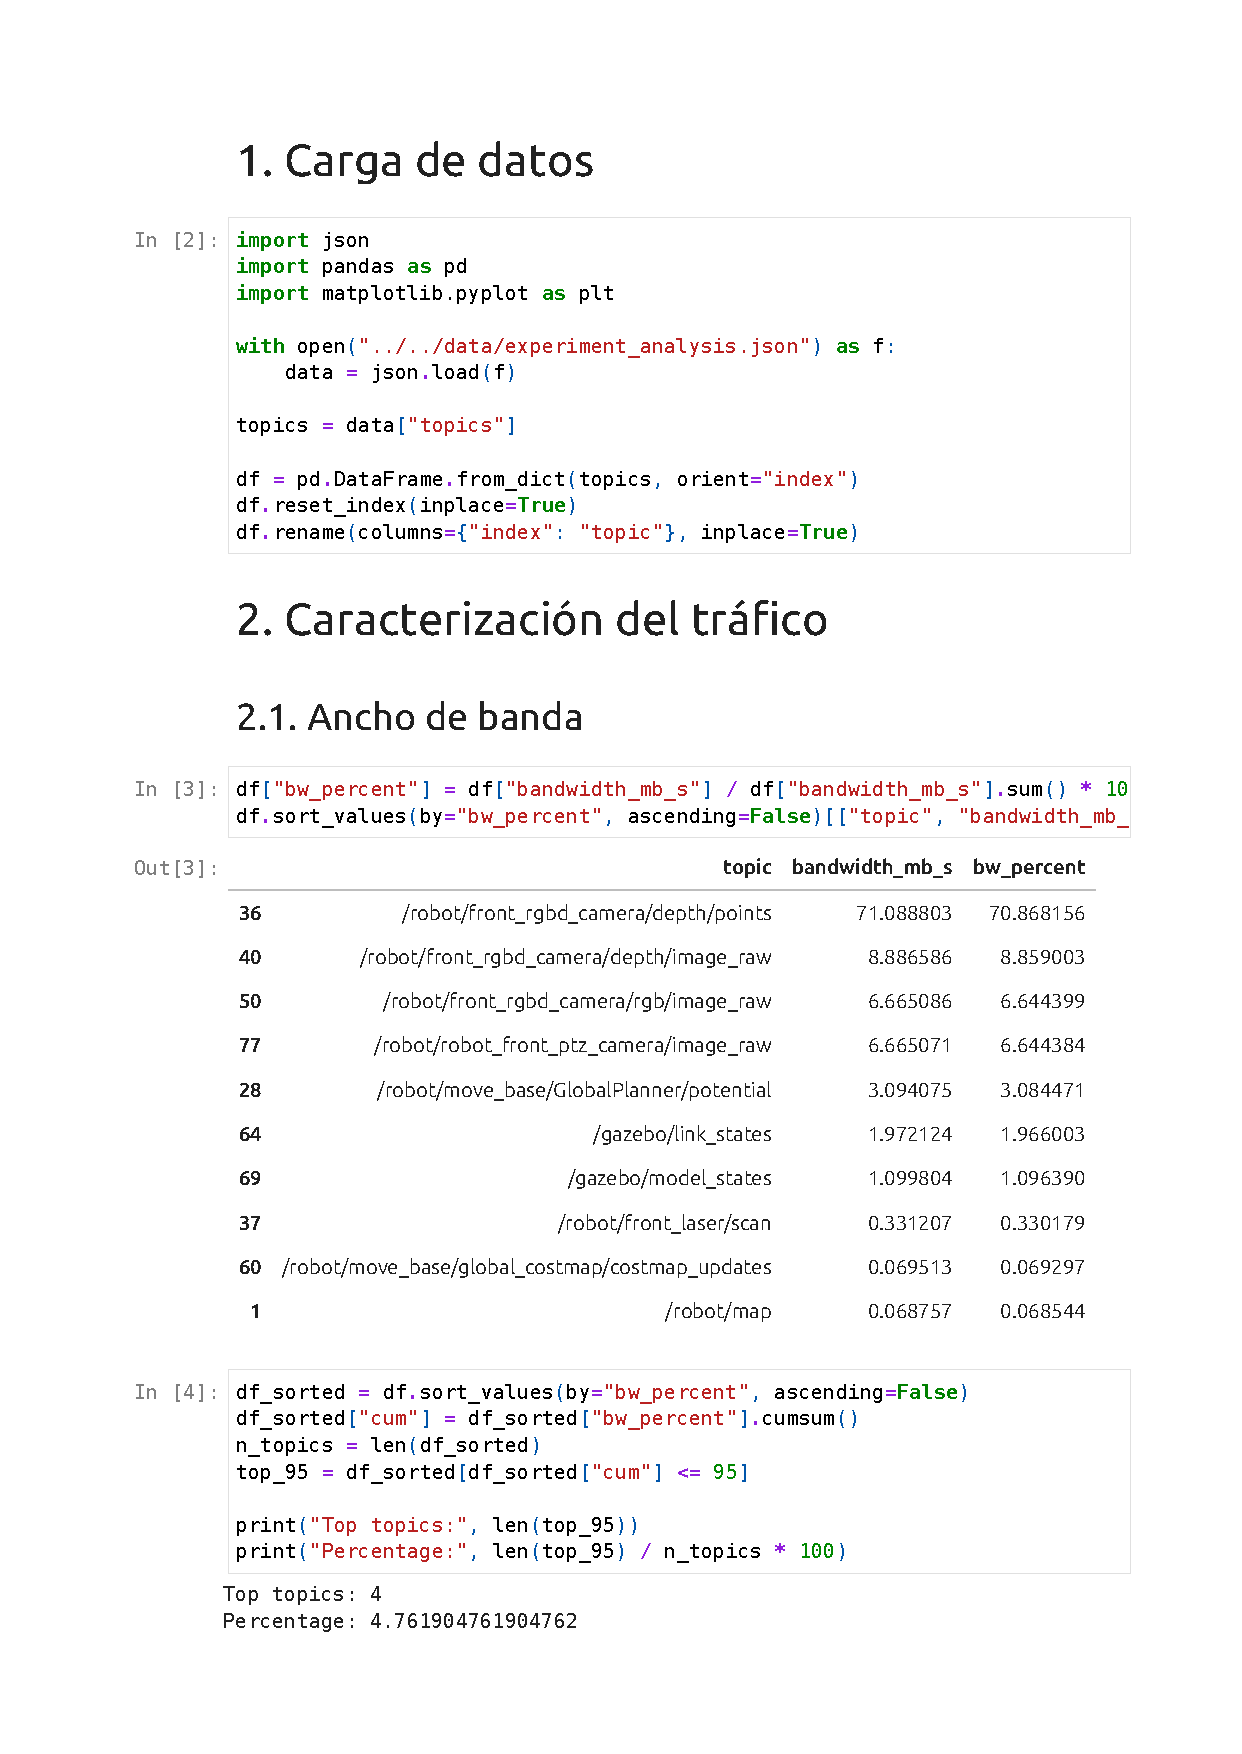
\includepdf[pages=-]{../scripts/analysis/robot_system_full_analysis.pdf}
\section{Análisis de la latencia en arquitectura centralizada}

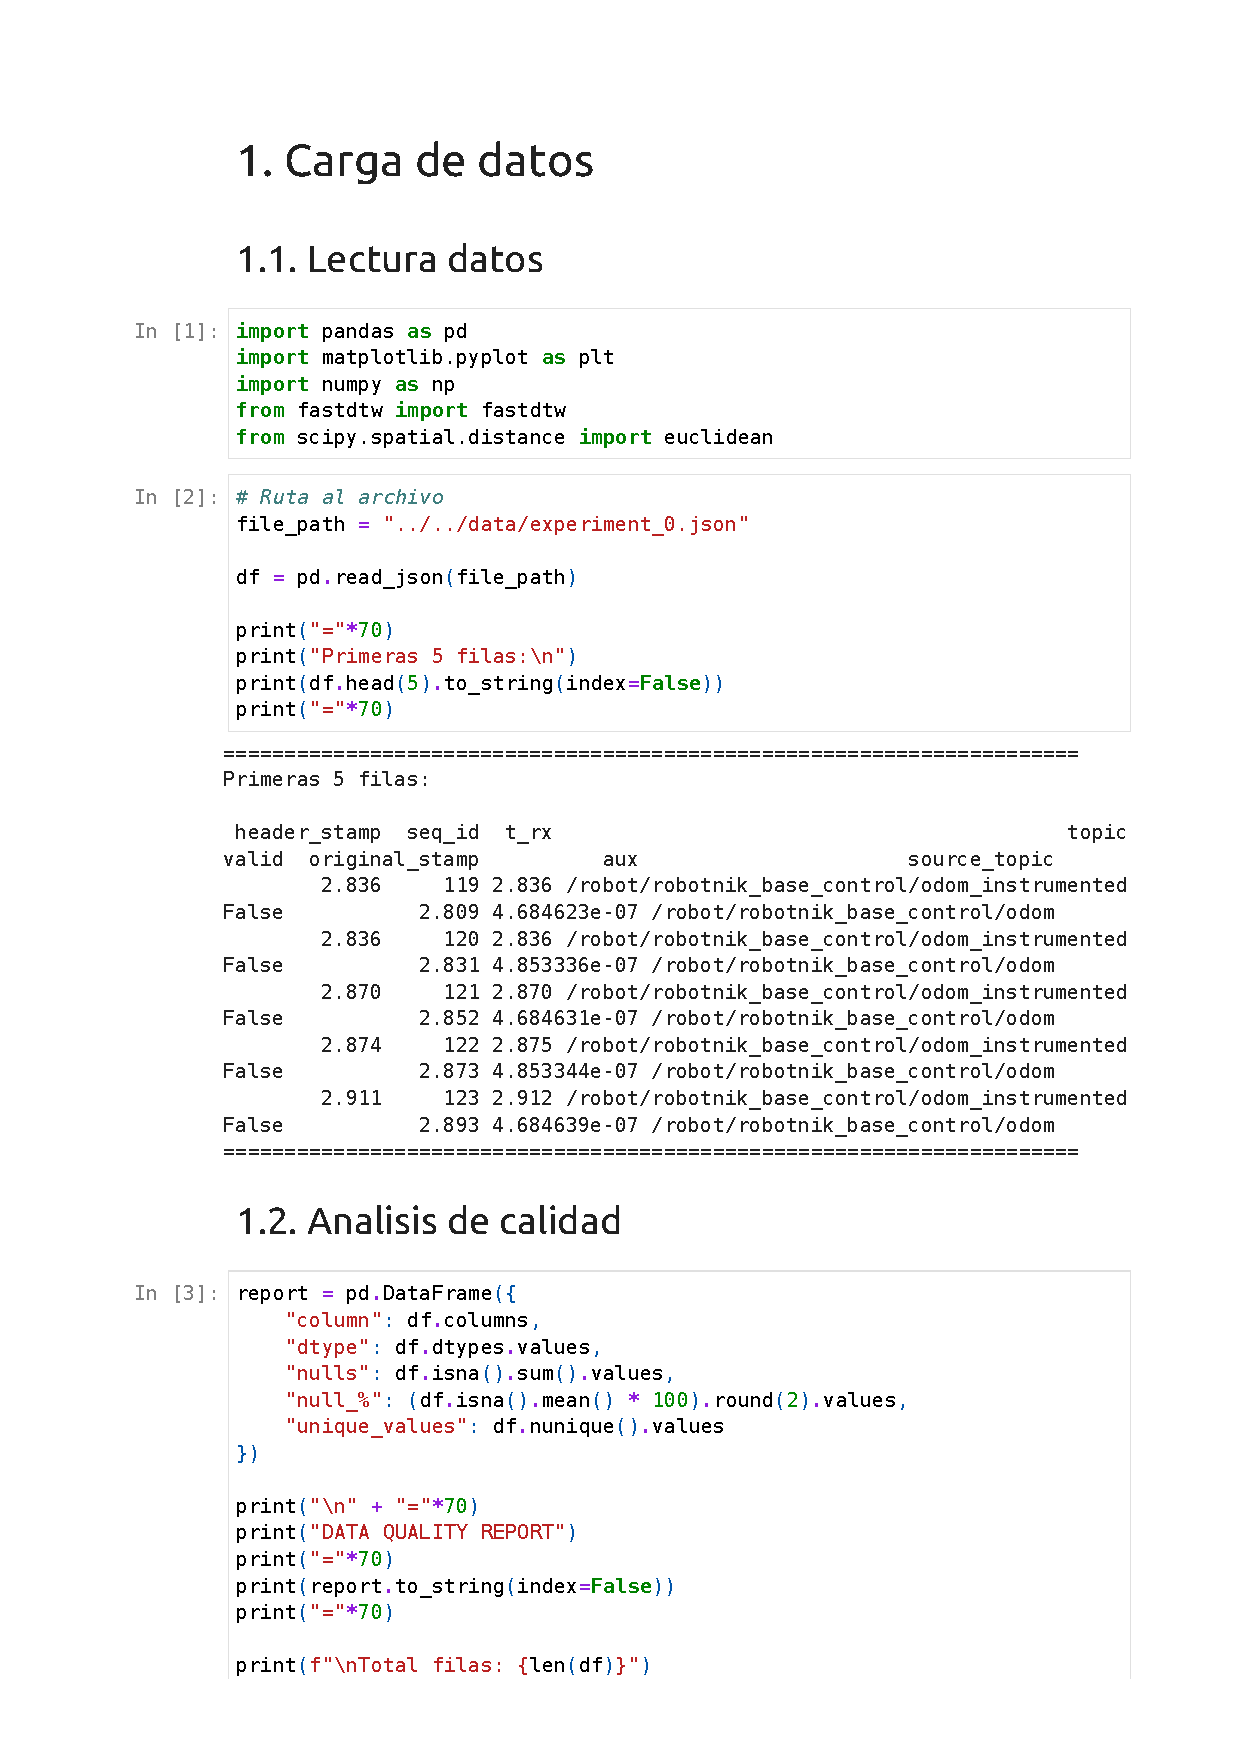
\includepdf[pages=-]{../scripts/analysis/robot_latency_analysis_centralized.pdf}




% ================================================================
% 08. BIBLIOGRAFIA
% ================================================================

\bibliographystyle{IEEEtran}
\bibliography{bibliography}

\end{document}